\documentclass[11pt]{article}
\usepackage[margin=1in]{geometry} 
\geometry{letterpaper}   

\usepackage{amssymb,amsfonts,amsmath,bbm,mathrsfs,stmaryrd}
\usepackage{xcolor}
\usepackage{url}
\usepackage{cancel}
%\usepackage{ulem}

\usepackage{enumerate}

%\usepackage{parskip}

\usepackage[colorlinks,
             linkcolor=black!75!red,
             citecolor=blue,
             pdfproducer={pdfLaTeX},
             pdfpagemode=None,
             bookmarksopen=true
             bookmarksnumbered=true]{hyperref}

\usepackage{tikz}
%\usetikzlibrary{arrows,decorations.pathreplacing,decorations.markings,shapes.geometric,through,fit,shapes.symbols,positioning}
\usetikzlibrary{arrows,calc,decorations.pathreplacing,decorations.markings,intersections,shapes.geometric,shapes,through,fit,shapes.symbols,positioning,decorations.pathmorphing}

\usepackage{braket}


%%% Theorems and references %%%
\usepackage[amsmath,thmmarks,hyperref]{ntheorem}
\usepackage{cleveref}

\creflabelformat{enumi}{#2(#1)#3}

\crefname{section}{Section}{Sections}
\crefformat{section}{#2Section~#1#3} 
\Crefformat{section}{#2Section~#1#3} 

\crefname{subsection}{\S}{\S\S}
\AtBeginDocument{%
  \crefformat{subsection}{#2\S#1#3}%
  \Crefformat{subsection}{#2\S#1#3}% 
}

\theoremstyle{plain}

\newtheorem{lemma}{Lemma}[section]
\newtheorem{proposition}[lemma]{Proposition}
\newtheorem{corollary}[lemma]{Corollary}
\newtheorem{theorem}[lemma]{Theorem}
\newtheorem{conjecture}[lemma]{Conjecture}
\newtheorem{question}[lemma]{Question}
\newtheorem{assumption}[lemma]{Assumption}


\theoremstyle{nonumberplain}
\newtheorem{theoremN}{Theorem}
\newtheorem{propositionN}{Proposition}
\newtheorem{corollaryN}{Corollary}


\theoremstyle{plain}
\theorembodyfont{\upshape}
\theoremsymbol{\ensuremath{\blacklozenge}}

\newtheorem{definition}[lemma]{Definition}
\newtheorem{example}[lemma]{Example}
\newtheorem{remark}[lemma]{Remark}
\newtheorem{convention}[lemma]{Convention}
\newtheorem{notation}[lemma]{Notation}

\crefname{definition}{definition}{definitions}
\crefformat{definition}{#2definition~#1#3} 
\Crefformat{definition}{#2Definition~#1#3} 

\crefname{ex}{example}{examples}
\crefformat{example}{#2example~#1#3} 
\Crefformat{example}{#2Example~#1#3} 

\crefname{remark}{remark}{remarks}
\crefformat{remark}{#2remark~#1#3} 
\Crefformat{remark}{#2Remark~#1#3} 

\crefname{convention}{convention}{conventions}
\crefformat{convention}{#2convention~#1#3} 
\Crefformat{convention}{#2Convention~#1#3} 

\crefname{notation}{notation}{notations}
\crefformat{notation}{#2notation~#1#3} 
\Crefformat{notation}{#2Notation~#1#3} 




\crefname{lemma}{lemma}{lemmas}
\crefformat{lemma}{#2lemma~#1#3} 
\Crefformat{lemma}{#2Lemma~#1#3} 

\crefname{proposition}{proposition}{propositions}
\crefformat{proposition}{#2proposition~#1#3} 
\Crefformat{proposition}{#2Proposition~#1#3} 

\crefname{corollary}{corollary}{corollaries}
\crefformat{corollary}{#2corollary~#1#3} 
\Crefformat{corollary}{#2Corollary~#1#3} 

\crefname{theorem}{theorem}{theorems}
\crefformat{theorem}{#2theorem~#1#3} 
\Crefformat{theorem}{#2Theorem~#1#3} 

\crefname{enumi}{}{}
\crefformat{enumi}{(#2#1#3)}
\Crefformat{enumi}{(#2#1#3)}

\crefname{assumption}{assumption}{Assumptions}
\crefformat{assumption}{#2assumption~#1#3} 
\Crefformat{assumption}{#2Assumption~#1#3} 

\crefname{equation}{}{}
\crefformat{equation}{(#2#1#3)} 
\Crefformat{equation}{(#2#1#3)}

%----------------Numbering equations---------------------

\numberwithin{equation}{section}
\renewcommand{\theequation}{\thesection-\arabic{equation}}


\theoremstyle{nonumberplain}
\theoremsymbol{\ensuremath{\blacksquare}}

\newtheorem{proof}{Proof}
\newcommand\pf[1]{\newtheorem{#1}{Proof of \Cref{#1}}}


\newcommand\bb[1]{{\mathbb #1}} 

\newcommand\bA{{\mathbb A}}
\newcommand\bB{{\mathbb B}}
\newcommand\bC{{\mathbb C}}
\newcommand\bD{{\mathbb D}}
\newcommand\bE{{\mathbb E}}
\newcommand\bF{{\mathbb F}}
\newcommand\bG{{\mathbb G}}
\newcommand\bH{{\mathbb H}}
\newcommand\bI{{\mathbb I}}
\newcommand\bJ{{\mathbb J}}
\newcommand\bK{{\mathbb K}}
\newcommand\bL{{\mathbb L}}
\newcommand\bM{{\mathbb M}}
\newcommand\bN{{\mathbb N}}
\newcommand\bO{{\mathbb O}}
\newcommand\bP{{\mathbb P}}
\newcommand\bQ{{\mathbb Q}}
\newcommand\bR{{\mathbb R}}
\newcommand\bS{{\mathbb S}}
\newcommand\bT{{\mathbb T}}
\newcommand\bU{{\mathbb U}}
\newcommand\bV{{\mathbb V}}
\newcommand\bW{{\mathbb W}}
\newcommand\bX{{\mathbb X}}
\newcommand\bY{{\mathbb Y}}
\newcommand\bZ{{\mathbb Z}}

\newcommand\cA{{\mathcal A}}
\newcommand\cB{{\mathcal B}}
\newcommand\cC{{\mathcal C}}
\newcommand\cD{{\mathcal D}}
\newcommand\cE{{\mathcal E}}
\newcommand\cF{{\mathcal F}}
\newcommand\cG{{\mathcal G}}
\newcommand\cH{{\mathcal H}}
\newcommand\cI{{\mathcal I}}
\newcommand\cJ{{\mathcal J}}
\newcommand\cK{{\mathcal K}}
\newcommand\cL{{\mathcal L}}
\newcommand\cM{{\mathcal M}}
\newcommand\cN{{\mathcal N}}
\newcommand\cO{{\mathcal O}}
\newcommand\cP{{\mathcal P}}
\newcommand\cQ{{\mathcal Q}}
\newcommand\cR{{\mathcal R}}
\newcommand\cS{{\mathcal S}}
\newcommand\cT{{\mathcal T}}
\newcommand\cU{{\mathcal U}}
\newcommand\cV{{\mathcal V}}
\newcommand\cW{{\mathcal W}}
\newcommand\cX{{\mathcal X}}
\newcommand\cY{{\mathcal Y}}
\newcommand\cZ{{\mathcal Z}}

\newcommand\fA{{\mathfrak A}}
\newcommand\fB{{\mathfrak B}}
\newcommand\fC{{\mathfrak C}}
\newcommand\fD{{\mathfrak D}}
\newcommand\fE{{\mathfrak E}}
\newcommand\fF{{\mathfrak F}}
\newcommand\fG{{\mathfrak G}}
\newcommand\fH{{\mathfrak H}}
\newcommand\fI{{\mathfrak I}}
\newcommand\fJ{{\mathfrak J}}
\newcommand\fK{{\mathfrak K}}
\newcommand\fL{{\mathfrak L}}
\newcommand\fM{{\mathfrak M}}
\newcommand\fN{{\mathfrak N}}
\newcommand\fO{{\mathfrak O}}
\newcommand\fP{{\mathfrak P}}
\newcommand\fQ{{\mathfrak Q}}
\newcommand\fR{{\mathfrak R}}
\newcommand\fS{{\mathfrak S}}
\newcommand\fT{{\mathfrak T}}
\newcommand\fU{{\mathfrak U}}
\newcommand\fV{{\mathfrak V}}
\newcommand\fW{{\mathfrak W}}
\newcommand\fX{{\mathfrak X}}
\newcommand\fY{{\mathfrak Y}}
\newcommand\fZ{{\mathfrak Z}}

\newcommand\fa{{\mathfrak a}}
\newcommand\fb{{\mathfrak b}}
\newcommand\fc{{\mathfrak c}}
\newcommand\fd{{\mathfrak d}}
\newcommand\fe{{\mathfrak e}}
\newcommand\ff{{\mathfrak f}}
\newcommand\fg{{\mathfrak g}}
\newcommand\fh{{\mathfrak h}}
%\newcommand\fi{{\mathfrak i}}
\newcommand\fj{{\mathfrak j}}
\newcommand\fk{{\mathfrak k}}
\newcommand\fl{{\mathfrak l}}
\newcommand\fm{{\mathfrak m}}
\newcommand\fn{{\mathfrak n}}
\newcommand\fo{{\mathfrak o}}
\newcommand\fp{{\mathfrak p}}
\newcommand\fq{{\mathfrak q}}
\newcommand\fr{{\mathfrak r}}
\newcommand\fs{{\mathfrak s}}
\newcommand\ft{{\mathfrak t}}
\newcommand\fu{{\mathfrak u}}
\newcommand\fv{{\mathfrak v}}
\newcommand\fw{{\mathfrak w}}
\newcommand\fx{{\mathfrak x}}
\newcommand\fy{{\mathfrak y}}
\newcommand\fz{{\mathfrak z}}


\newcommand\fgl{\mathfrak{gl}}
\newcommand\fsl{\mathfrak{sl}}
\newcommand\fsp{\mathfrak{sp}}


\newcommand\ol{\overline}
\newcommand\wt{\widetilde}

\newcommand\md{\mathrm{Mod}}

\newcommand\1{{\bf 1}}


%%%%%%%%%%%%%%%%%%% simple math operators %%%%%%%%%%%%%%%%%%%
\DeclareMathOperator{\id}{id}
\DeclareMathOperator{\End}{\mathrm{End}}
\DeclareMathOperator{\Hom}{\mathrm{Hom}}
\DeclareMathOperator{\pr}{\mathrm{Prob}}
\DeclareMathOperator{\orb}{\mathrm{Orb}}


\DeclareMathOperator{\cact}{\cat{CAct}}
\DeclareMathOperator{\wact}{\cat{WAct}}

\DeclareMathOperator{\ot}{\leftarrow}

%%%%%%%%%%%%%%%%%%%%%%%%%%%%%%%%%%%%%%%%%%%%%%%%%%%%%%%%%%
%%% align* numbering %%%

\newcommand\numberthis{\addtocounter{equation}{1}\tag{\theequation}}


%%%%%%%%%%%%%%%%%%%%%%%%%%%%%%%%%%%%%%%%%%%%%%%%%%%%%%%%%%
%%% misc %%%

\newcommand{\define}[1]{{\em #1}}

\newcommand{\cat}[1]{\textsc{#1}}
\newcommand\mathify[2]{\newcommand{#1}{\cat{#2}}}
\newcommand\spr[1]{\cite[\href{https://stacks.math.columbia.edu/tag/#1}{Tag {#1}}]{stacks-project}}
\newcommand{\qedhere}{\mbox{}\hfill\ensuremath{\blacksquare}}


\renewcommand{\square}{\mathrel{\Box}}

\newcommand{\mike}[1]{{\bf \color{red} **{#1}**}}
\newcommand{\alex}[1]{{\bf \color{green} **{#1}**}}
\newcommand{\amaury}[1]{{\bf \color{cyan} **{#1}**}}


\newcommand\Section[1]{\section{#1}\setcounter{lemma}{0}}



%%%%%

\title{Universal tensor categories generated by dual pairs}
\author{Alexandru Chirvasitu and Ivan Penkov}

%\subjclass[2010]{102000}

\begin{document}

\date{}


\newcommand{\Addresses}{{% additional braces for segregating \footnotesize
  \bigskip
  \footnotesize

  \textsc{Department of Mathematics, University at Buffalo, Buffalo,
    NY 14260-2900, USA}\par\nopagebreak
  \textit{E-mail address}: \texttt{achirvas@buffalo.edu}

  \medskip

  \textsc{Jacobs University Bremen, Campus Ring 1, 28759 Bremen, Germany}\par\nopagebreak
  \textit{E-mail address}: \texttt{i.penkov@jacobs-university.de}  

% %   \medskip
% %   
% %   \textsc{Department of Mathematics, institution,
% %     address}\par\nopagebreak \textit{E-mail address}:
% %   \texttt{??}
% % 
}}


\maketitle

\begin{abstract}
  Let $V_*\otimes V\rightarrow\mathbb{C}$ be a non-degenerate pairing of countable-dimensional complex vector spaces $V$ and $V_*$. The Mackey Lie algebra $\mathfrak{g}=\mathfrak{gl}^M(V,V_*)$ corresponding to this pairing consists of all endomorphisms $\varphi$ of $V$ for which the space $V_*$ is stable under the dual endomorphism $\varphi^*: V^*\rightarrow V^*$. We study the tensor Grothendieck category $\mathbb{T}$ generated by the $\mathfrak{g}$-modules $V$, $V_*$ and their algebraic duals $V^*$ and $V^*_*$. The category $\bT$ is an analogue of categories considered in prior literature, the main difference being that the trivial module $\mathbb{C}$ is no longer injective in $\mathbb{T}$. We describe the injective hull $I$ of $\mathbb{C}$ in $\mathbb{T}$, and show that the category $\mathbb{T}$ is Koszul. In addition, we prove that $I$ is endowed with a natural structure of commutative algebra. We then define another category $_I\mathbb{T}$ of objects in $\mathbb{T}$ which are free as $I$-modules. Our main result is that the category ${}_I\mathbb{T}$ is also Koszul, and moreover that ${}_I\mathbb{T}$ is universal among abelian $\mathbb{C}$-linear tensor categories generated by two objects $X$, $Y$ with fixed subobjects $X'\hookrightarrow X$, $Y'\hookrightarrow Y$ and a pairing $X\otimes Y\rightarrow \text{\textbf{1}}$ where \textbf{1} is the monoidal unit. We conclude the paper by discussing the orthogonal and symplectic analogues of the categories $\mathbb{T}$ and ${}_I\mathbb{T}$.
\end{abstract}

\noindent {\em Key words:} Mackey Lie algebra, tensor module, monoidal category, Koszulity, Grothendieck category, semi-artinian



\vspace{.5cm}


\noindent{MSC 2020: }17B65; 17B10; 18M05; 18E10; 16T15; 16S37

\tableofcontents


%%%%%%%%%%%%%%%%%%%%%%%%%%%%%%%%%%%%%%%%%%%%%%%%%%%%%%%%%%%%%%%%%%%%%%%%%%%%%%%%%%%%%%%%%%%%%%%%%%%%%%%%%%%%%%%%%%
%%%%%%%%%%%%%%%%%%%%%%%%%%%%%%%%%%%%%%%%%%%%%%%%%%%%%%%%%%%%%%%%%%%%%%%%%%%%%%%%%%%%%%%%%%%%%%%%%%%%%%%%%%%%%%%%%%
\section{Introduction}


A tensor category for us is a symmetric, not necessarily rigid, $\mathbb{C}$-linear monoidal abelian category. In this paper we construct and study a tensor category which is universal as a tensor category generated by two objects $X$, $Y$ with fixed subobjects $X'\hookrightarrow X$, $Y'\hookrightarrow Y$ and endowed with a pairing $X\otimes Y\rightarrow {\bf 1}$, the object ${\bf 1}$ being the monoidal unit.

The simpler problem of constructing a universal tensor category generated just by two objects $X$, $Y$ endowed with pairing $X\otimes Y\rightarrow {\bf 1}$ was solved several years ago, and explicit constructions of such a category are given in \cite{SS} and \cite{DPS}. The construction in \cite{DPS} realizes this category as a category $\bT_{\fsl(\infty)}$ of representations of the Lie algebra $\fsl(\infty)$, choosing $X$ as the natural $\fsl(\infty)$-module $V$, and $Y$ as its restricted dual $V_*$. Motivated mostly by a desire to understand better the representation theory of the Lie algebra $\fsl(\infty)$, in \cite{PS1} a larger category was constructed, denoted $\widetilde{Tens}_{\fsl(\infty)}$, which contains also the algebraic dual modules $V^*$ and $V_*^*$. It is clear that the category $\widetilde{Tens}_{\fsl(\infty)}$ has a completely different flavor as its objects have uncountable length while $\bT_{\fsl(\infty)}$ is a finite-length category.

However, in \cite{PS2} the observation was made that the four representations $V$, $V_*$, $V^*$, $V_*^*$ generate a finite-length tensor category $\bT^{4}_{\mathfrak{gl}^M(V,V_*)}$ over the larger Lie algebra $\mathfrak{gl}^M(V,V_*)$, see Section \ref{se.prel}. We call this latter Lie algebra a Mackey Lie algebra as its introduction has been inspired by G. Mackey's work \cite{M}. The simple objects of $\bT^{4}_{\mathfrak{gl}^M(V,V_*)}$ were determined in \cite{Chi14}. Furthermore, in \cite{us0} the tensor category $\bT^{3}_{\mathfrak{gl}^M(V,V_*)}$, generated by $V$, $V_*$, and  $V^*$, was studied in detail. It was proved that $\bT^{3}_{\mathfrak{gl}^M(V,V_*)}$ is Koszul, and it was established that $\bT^{3}_{\mathfrak{gl}^M(V,V_*)}$ is universal as a tensor category generated by two objects $X$, $Y$ with a pairing $X\otimes Y\rightarrow {\bf 1}$, such that $X$ has a subobject $X'\hookrightarrow X$. Later, a vast generalization of the results of \cite{us0} was given in \cite{us1}: here a universal tensor category with two objects $X$, $Y$, a paring $X\otimes Y\rightarrow {\bf 1}$ and an arbitrary (possibly transfinite) fixed filtration of $X$ was realized as category of representations of a certain large Lie algebra.

A main difference of the category  $\bT^{4}_{\mathfrak{gl}^M(V,V_*)}$ with previously studied categories is that, as we show in the present paper, the injective hulls of simple objects are not objects of  $\bT^{4}_{\mathfrak{gl}^M(V,V_*)}$ but of a colimit-completion of $\bT^{4}_{\mathfrak{gl}^M(V,V_*)}$ which we denote simply by $\bT$. In particular, the trivial module has an injective hull $I$ in $\bT$ of infinite Loewy length, i.e. with an infinite socle filtration. Moreover, remarkably, $I$ has the structure of a commutative algebra. 

This leads us to the idea of considering the category ${}_I\bT$ of $I$-modules internal to $\bT$. The morphisms in this new category are morphisms of $\fgl^M(V,V_*)$-modules as well as of $I$-modules. The simple objects of ${}_I\bT$ are of the form $I\otimes M$ where $M$ is a simple module in $\bT$. 

A culminating result of the present paper is that the category ${}_I\bT$ has the universality property stated in the first paragraph of this introduction. The pairs $X'\hookrightarrow X$ and $Y'\hookrightarrow Y$ are realized respectively as $I \otimes V_*\subset I \otimes V^* $ and $I \otimes V\subset I \otimes V_*^*$, $I$ is the unity object in ${}_I\bT$, and the tensor product in ${}_I\bT$ is $\otimes_I$.

 Finally, in Section \ref{se:bcd} we study analogues of the tensor categories $\bT_{\fo(\infty)}$ and $\bT_{\fs\fp(\infty)}$ considered in \cite{DPS} and \cite{SS}. Consider a tensor category generated by a single object $X$ with a subobject $X'\hookrightarrow X$ and a pairing $X\otimes X\rightarrow \text{\textbf{1}}$. After identifying $V_*$ and $V$, our construction of the category ${}_I\bT$ yields a universal tensor category also in this setting. However, one can assume in addition that the pairing 
$X\otimes X\rightarrow \text{\textbf{1}}$ is symmetric or antisymmetric, which leads to new universality problems for tensor categories. %as the pairing $X\otimes_I X \rightarrow \text{\textbf{1}}$ for $X=I\otimes V=I\otimes V_*$ in the already constructed category $_I \bT$ is not symmetric or antisymmetric.
 With this in mind, we introduce %that these new universality problems can be solved by introducing categories
  $\bT^2_{\fo(V)}$ and $\bT^2_{\fs\fp(V)}$ where $\fo(V)$ and $\fs\fp(V)$ are respective orthogonal and symplectic Lie algebras of a countable-dimensional vector space $V$. In analogy with our previous constructions, we then produce appropriate categories $_{I'} \bT^2$ for $I'=I_{\fo(V)}$ and $I'=I_{\fs\fp(V)}$ and prove that these latter categories are universal in the respective new settings. Moreover, the categories ${}_{I_{\fo(V)}}\bT^2$ and ${}_{I_{\fs\fp(V)}}\bT^2$ are canonically equivalent as monoidal categories.


%%%%%%%%%%%%%%%%%%%%%%%%%%%%%%%%%%%%%%%%%%%%%%%%%%%%%%%%%%%%%%%%%%%%%%%%%%%%%%%%%%%%%%%%%%%%%%%%%%%%%%%%%%%%%%%%%%
\subsection*{Acknowledgements}

We thank a referee for a thorough reading of an earlier draft of the paper and for excellent suggestions. A.C. was partially supported by NSF grants DMS-1801011 and DMS-2001128. I.P. was partially supported by DFG grants PE 980-7/1 and PE 980-8/1. 


%%%%%%%%%%%%%%%%%%%%%%%%%%%%%%%%%%%%%%%%%%%%%%%%%%%%%%%%%%%%%%%%%%%%%%%%%%%%%%%%%%%%%%%%%%%%%%%%%%%%%%%%%%%%%%%%%%
%%%%%%%%%%%%%%%%%%%%%%%%%%%%%%%%%%%%%%%%%%%%%%%%%%%%%%%%%%%%%%%%%%%%%%%%%%%%%%%%%%%%%%%%%%%%%%%%%%%%%%%%%%%%%%%%%%
\section{Preliminaries}\label{se.prel}

\subsection{Notation}
All vector spaces are defined over $\bC$ (more generally, we could work over an algebraically closed field of characteristic zero); similarly, all abelian categories and all functors between such are assumed $\bC$-linear, and we refer to \cite{groth} for general background on abelian/additive categories.

% % 
% % \begin{notation}\label{not:mor}
% %   \textcolor{red}{\cancel{For objects $x,y\in \cC$ in a category we write}
% %   \begin{align*}
% %     \cancel{(y\ot x)_\cC} &\cancel{:= \Hom_{\cC}(x,y)}\\
% %     \cancel{(x)_\cC} &\cancel{:= \End_{\cC}(x),}\\
% %   \end{align*}
% %   \cancel{or simply $(y\ot x)$ and $(x)$ respectively when the category is understood. }}
% % \end{notation}
% % 

By $S^k X$ and $\Lambda^k X$ we denote respectively the $k$-th symmetric and exterior powers of a vector space $X$, and $S_n$ stands for the symmetric group on $n$ letters.

Once and for all we fix a non-degenerate pairing $V_*\otimes_{\bC} V\rightarrow \bC$ of countable-dimensional vector spaces $V$ and $V_*$. This pairing defines embeddings $V_*\subset V^*$, $V\subset V^*_*$, where $V^*=\Hom_{\bC}(V,\bC)$, $V_*^*=\Hom_{\bC}(V_*,\bC)$. For any vector space $M$ we set $M^*=\Hom_{\bC}(M,\bC)$. We abbreviate $\otimes_{\bC}$ as $\otimes$. By $\otimes$ we denote also tensor product in abstract tensor categories in the hope that this will cause no confusion.

Except in Section \ref{se:bcd}, $\fg$ will be the {\it Mackey Lie algebra} $\fgl^M$ {$(V,V_*)$} of \cite{PS2} associated to the pairing $V_*\otimes V\to \bC$. By definition, $$\fgl^M(V,V_*)=\{ \varphi\in \End V \mid \varphi^*(V_*)\subset V_*\},$$ where $\varphi^*:V^*\rightarrow V^*$ is the operator dual to $\varphi$. We will describe $\fg$ explicitly as a Lie algebra of infinite matrices shortly. 

We set
\begin{equation*}
  W_*:=V^*/V_*,\quad W := V_*^*/V\quad\text{and}\quad F:=W_*\otimes W.  
\end{equation*}

There is an extension
\begin{equation}\label{eq:exatseqQ}
  0\to \bC\to Q\to F\to 0
\end{equation}
where $Q$ is defined as the quotient of $V^*\otimes V_*^*$ by the sum of the kernels of the pairings
\begin{equation*}
  V^*\otimes V\to \bC\quad \text{and}\quad V_*\otimes V_*^*\to \bC.
\end{equation*}
In Proposition \ref{pr.ann} below we prove that the extension \Cref{eq:exatseqQ} is non-splitting.
% % \textcolor{red}{\xcancel{$\bT$ will denote the four-diagram category that is the focus of the present paper (see \Cref{subse:ord-cat} below),} $\bT_s$ the largest tensor subquotient-closed subcategory generated by the canonical extension $Q$ of $F$ by $\bC$ described above, and $\bT_f$ the intermediate subquotient-closed tensor subcategory (containing $\bT_s$ and contained in $\bT$) generated by $W$ and $W_*$.}
% %

% % We also work with the Grothendieck closures of these categories, consisting of representations of the Mackey Lie algebra $\fg=\fg^M$ that are unions of objects in the respective categories; the operation of Grothendieck closure will be denoted by an overline, as in $\overline{\bT}$.
% %

We model the actions of $\fg$ on various modules mentioned above as follows:

\begin{itemize}
\item[$-$] $V_*^*$ consists of infinite column vectors with entries indexed by $\bN=\{0,1,\cdots\}$.
\item[$-$] $V\subset V^*_*$ consists of {\it finite} ({\it or finitary}) column vectors, i.e. those with at most finitely many non-zero entries.
\item[$-$] Dually, $V^*$ consists of $\bN$-indexed infinite row vectors.
\item[$-$] The elements of $V_*\subset V^*$ are precisely the finite row vectors. 
\item[$-$] $\fg$ consists of $\bN\times \bN$-matrices with finite rows and columns, acting on $V_*^*$ by left multiplication.
\item[$-$] Similarly, $\fg$ acts on $V^*$ as minus right multiplication. 
\item[$-$] $V^*\otimes V^*_*$ consists of finite-rank $\bN\times \bN$ matrices with infinite rows and columns, acted upon by $\fg$ by commutation.
\end{itemize}

We will frequently make use of Schur functors $\mathbb{S}_{\lambda}$ attached to Young diagrams $\lambda$. Often we write $X_{\lambda}$ instead of $\bS_{\lambda} X$ for a vector space $X$. Moreover, $S^k X=\mathbb{S}_{\rho} X$, $\Lambda^k X=\mathbb{S}_{\gamma}X$, where $\rho$, $\gamma$ are respectively a row and a column with $k$ boxes.

For Young diagrams $\lambda$, $\mu$, $\nu$ and $\pi$ we write
\begin{align*}
  L_{\lambda,\mu,\nu,\pi}&:=W_{*\lambda}\otimes V_{\mu,\nu}\otimes W_{\pi}\label{eq:s}\numberthis, \\
  J_{\lambda,\mu,\nu,\pi}&:=W_{*\lambda}\otimes V^*_{\mu}\otimes V^*_{\nu}\otimes W_{\pi},
\end{align*}
and similarly, for non-negative integers $l,m,n,p$ we set
\begin{align*}
  L_{l,m,n,p}&:=W_*^{\otimes l}\otimes V_{m,n}\otimes W^{\otimes p},\\
  J_{l,m,n,p}&:=W_*^{\otimes l}\otimes V^{*\otimes m}\otimes V_*^{*\otimes n}\otimes W^{\otimes p}\label{eq:j}\numberthis,
\end{align*}
where $V_{m,n}$ is the socle of $V^{*\otimes m}\otimes V^{\otimes n}$, i.e.
\begin{equation*}
  V_{m,n}=\bigoplus_{|\mu|=m,|\nu|=n}V_{\mu,\nu}^{m_{\mu,\nu}}
\end{equation*}
for appropriate multiplicities $m_{\mu,\nu}$. Here $|\lambda|$ denotes the degree (number of boxes) of a Young diagram $\lambda$. Finally, for any subscript $s$ of the form $(\bullet,\bullet,\bullet,\bullet)$ we set
\begin{equation}\label{eq:13}
  I_s:=I\otimes J_s,
\end{equation}
where $I$ is the object constructed below in \Cref{se.a}. 

\begin{definition}\label{def.thk}
  We refer to objects involving only the two outside diagrams $\lambda$ and $\pi$ as {\it purely thick} %(or {\it purely thick} for emphasis) 
  and those involving only the two middle diagrams as {\it thin}. Everything else is {\it mixed}. 
\end{definition}

It is essential to recall Corollary 4.3 in \cite{us0} which claims that $L_{\lambda,\mu,\nu,\pi}$ is a simple $\fg$-module, and implies that $L_{l,m,n,p}$ is a semisimple $\fg$-module.

The following remark will be used implicitly and repeatedly: given a short exact sequence
\begin{equation*}
  0\to x'\to x\to x''\to 0
\end{equation*}
in a tensor abelian category, the symmetric power $S^kx$ has a filtration
\begin{equation*}
  0=F_{-1}\subset F_0\subset \cdots\subset F_n = S^k x
\end{equation*}
with isomorphisms
\begin{equation*}
  F_j/F_{j-1} \cong S^{k-j} x'\otimes S^jx'' \text{ for }  0\le j\le k. 
\end{equation*}


%%%%%%%%%%%%%%%%%%%%%%%%%%%%%%%%%%%%%%%%%%%%%%%%%%%%%%%%%%%%%%%%%%%%%%%%%%%%%
\subsection{Plethysm}\label{subse:plet}

%We will frequently make use of Schur functors $\mathbb{S}_{\lambda}$ attached to Young diagrams $\lambda$. Then $S^k \bullet=\mathbb{S}_{\lambda} \bullet$, $\Lambda^k \bullet=\mathbb{S}_{\mu}\bullet$, where $\lambda,\mu$ are respectively a row and a column with $k$ boxes.

Given that $F=W\otimes W_*$ and we have to work with symmetric and exterior powers of $F$, we will have to understand how such powers decompose as direct sums of objects of the form $\mathbb{S}_{\lambda}W\otimes \mathbb{S}_{\mu}W_*$. The result applies to a tensor product $W\otimes W_*$ in {\it any} $\bC$-linear tensor category, so we work in this generality throughout the present subsection.

We call a partition $\lambda$ {\it special} if it satisfies the condition: all hooks of $\lambda$ whose corner lies on the diagonal of $\lambda$ have horizontal and vertical arms (not counting the corner) of length $\mu_i-1$ and $\mu_i$, respectively, where $\mu_1> \mu_2 > \ldots > 0$ is a partition. We now recall the following result.

\begin{proposition}\label{pr.plth}
  Let $x$ and $y$ be two objects in a $\bC$-linear tensor category. We have the following decompositions:
  \begin{enumerate}[(a)]
  \item\label{item:1} $S^k(x\otimes y)$ is the direct sum of all objects of the form $\mathbb{S}_{\lambda}x\otimes \mathbb{S}_{\lambda}y$ as $\lambda$ ranges over all Young diagrams of degree $k$.
  \item\label{item:2} $\Lambda^k(x\otimes y)$ is the direct sum of all objects of the form $\mathbb{S}_{\lambda}x\otimes \mathbb{S}_{\lambda^{\perp}}y$ as $\lambda$ ranges over all Young diagrams of degree $k$, where $\lambda^{\perp}$ denotes the conjugate partition.
  \item\label{item:10} $S^k S^2 x$ is the direct sum of all $\bS_{\lambda}x$ for partitions $\lambda$ of degree $2k$ with even parts , i.e. {\it even partitions}. 
  \item\label{item:11} $S^k \Lambda^2 x$ is $\bigoplus_{\substack{\text{even }\lambda \\ |\lambda|=2k}}\bS_{\lambda^{\perp}}x$.
  \item\label{item:12} $\Lambda^k\Lambda^2 x$ is $\bigoplus_{\substack{\text{special }\lambda \\ |\lambda|=2k}}\bS_{\lambda}x$.
  \item\label{item:13} $\Lambda^k S^2 x$ is $\bigoplus_{\substack{\text{special }\lambda \\ |\lambda|=2k}}\bS_{\lambda^{\perp}}x$.    
  \end{enumerate}
\end{proposition}
\begin{proof}
  (\labelcref{item:1}) and (\labelcref{item:2}) are reformulations of the Cauchy identities in \cite[(6.2.8)]{ss-intro}. %which in the symmetric case say that the two-variable Schur functor $S^k(\bullet\otimes \bullet)$ decomposes as
  %\begin{equation*}
   % S^k(\bullet\otimes\bullet)\cong \bigoplus_{|\lambda|=k}(\mathbb{S}_\lambda\bullet)\otimes (\mathbb{S}_\lambda\bullet);
  %\end{equation*}
  %there is an obvious analogue for exterior powers.
  The other four points paraphrase \cite[Example I.8.6]{macd-bk}.
\end{proof}

%%%%%%%%%%%%%%%%%%%%%%%%%%%%%%%%%%%%%%%%%%%%%%%%%%%%%%%%%%%%%%%%%%%%%%%%%%%%%
\subsection{Ordered Grothendieck categories}\label{sec:orderedgrothendieckcat}

We recall the following notion from \cite[Definition 2.3]{us1}.

\begin{definition}\label{def.ord-gr}
  Let $(\cP,\preceq)$ be a poset. An {\it ordered Grothendieck category} with underlying order $(\cP,\preceq)$ is a Grothendieck category $\cC$ together with objects $X_s$, $s\in \cP$ so that the following conditions hold.

\begin{enumerate}[(a)]
\item\label{item:3} The objects $X_s$ are {\it semi-artinian}, in the sense that all of their non-zero quotients have non-zero socles.
%\item\label{item:4} $(\cP,\preceq)^{op}$ is well-ordered (i.e. every non-empty totally ordered subset has a largest element with respect to $\preceq$).
\item\label{item:5} Every object in $\cC$ is a subquotient of a direct sum of copies of various $X_s$.
\item\label{item:6} The simple subobjects in
  \begin{equation}\label{eq:14}
    \cS_s:=\{\text{isomorphism classes of simples in }\mathrm{soc}X_s\}
  \end{equation}
  are mutually non-isomorphic for distinct $s$ and they exhaust the simples in $\cC$.
\item\label{item:7} Simple subquotients of $X_s$ outside the socle $\mathrm{soc}X_s$ are in the socle of some $X_t$, $t\prec s$. 
\item\label{item:8} Each $X_s$ is a direct sum of objects with simple socle.
\item\label{item:9} Let $t\prec s$. The maximal subobject $X_{s\succ t}\subset X_{s}$ whose simple constituents belong to various $\cS_r$ for $s\succeq r\not\preceq t$ is the common kernel of a family of morphisms $X_s\to X_t$.
\end{enumerate}
\end{definition}

Ordered Grothendieck categories are well behaved in a number of ways. For instance (\cite[Corollary 2.6]{us1}):

\begin{proposition}
  The indecomposable injective objects in an ordered Grothendieck category $\cC$ are, up to isomorphism, precisely the indecomposable summands of the objects $X_s$ in \Cref{def.ord-gr}.  \qedhere
\end{proposition}

Recall (\cite[\S 3.2]{us0} or \cite[Definition 2.8]{us1}):

\begin{definition}\label{def:defect}
  For two elements $i\prec j$ in $\cP$ the {\it defect} $d(i,j)$ is the supremum of the set of non-negative integers $q$ for which we can find a chain
  \begin{equation*}
    i=i_0\prec \cdots\prec i_q=j.
  \end{equation*}
We put also $d(i,i):=0$. In the context of an ordered Grothendieck category as in \Cref{def.ord-gr} we adopt the simplified notation $d(S,T)$ for $d(s,t)$ when $S\in \cS_s$ and $T\in \cS_t$.  
\end{definition}

% % 
% %   We focus on \labelcref{item:1}, since the two proofs largely run in parallel. We want to argue that the map
% %   \begin{equation*}
% %     (x\otimes y)^{\otimes n} \to \bigoplus_{|\lambda|=n}S_\lambda x\otimes S_\lambda y
% %   \end{equation*}
% %   with $\lambda$ component
% %   \begin{equation*}
% %  \begin{tikzpicture}[auto,baseline=(current  bounding  box.center)]
% %   \path[anchor=base] (0,0) node (1) {$(x\otimes y)^{\otimes n}$} +(3,0) node (2) {$x^{\otimes n}\otimes y^{\otimes n}$} +(7,0) node (3) {$S_\lambda x\otimes S_\lambda y$};
% %   \draw[->] (1) to[bend left=0] node[pos=.5,auto] {$\scriptstyle \cong$} (2);
% %   \draw[->] (2) to[bend left=0] node[pos=.5,auto] {$\scriptstyle c_\lambda\otimes c_\lambda$} (3);
% %  \end{tikzpicture}
% % \end{equation*}
% % induces the desired isomorphism 
% % \begin{equation*}
% %   S^n(x\otimes y) \cong \bigoplus_{|\lambda|=n}S_\lambda x\otimes S_\lambda y,
% % \end{equation*}
% % where $c_\lambda\in \bC S_n$ denotes the Young symmetrizer associated to the diagram $\lambda$.
% % 
% % That this is indeed the case for finite-dimensional vector spaces $x$ and $y$ regarded as modules over $\fgl(x)\oplus \fgl(y)$ is a consequence of \cite[Theorem 4.1.1]{br}, and the conclusion follows in general by taking filtered colimits over the finite-dimensional subspaces of $x$ ad $y$ and noting that Schur functors commute with filtered colimits.
% % 



% % 
% % \begin{proposition}\label{pr.plth}
% %   Let $x$ and $y$ be two objects in a $\bC$-linear tensor category. We have the following decompositions:
% %   \begin{enumerate}[(a)]
% %   \item\label{item:1} $S^n(x\otimes y)$ is the direct sum of all objects of the form $S_{\lambda}x\otimes S_{\lambda}y$ as $\lambda$ ranges over all Young diagrams with $n$ boxes.
% %   \item\label{item:2} $\Lambda^n(x\otimes y)$ is the direct sum of all objects of the form $S_{\lambda}x\otimes S_{\lambda^{\perp}}y$ as $\lambda$ ranges over all Young diagrams with $n$ boxes, where $\lambda^{\perp}$ denotes the conjugate partition.
% %   \end{enumerate}
% % \end{proposition}
% % \begin{proof}
% %   We focus on \labelcref{item:1}, since the two proofs largely run in parallel. We want to argue that the map
% %   \begin{equation*}
% %     (x\otimes y)^{\otimes n} \to \bigoplus_{|\lambda|=n}S_\lambda x\otimes S_\lambda y
% %   \end{equation*}
% %   with $\lambda$ component
% %   \begin{equation*}
% %  \begin{tikzpicture}[auto,baseline=(current  bounding  box.center)]
% %   \path[anchor=base] (0,0) node (1) {$(x\otimes y)^{\otimes n}$} +(3,0) node (2) {$x^{\otimes n}\otimes y^{\otimes n}$} +(7,0) node (3) {$S_\lambda x\otimes S_\lambda y$};
% %   \draw[->] (1) to[bend left=0] node[pos=.5,auto] {$\scriptstyle \cong$} (2);
% %   \draw[->] (2) to[bend left=0] node[pos=.5,auto] {$\scriptstyle c_\lambda\otimes c_\lambda$} (3);
% %  \end{tikzpicture}
% % \end{equation*}
% % induces the desired isomorphism 
% % \begin{equation*}
% %   S^n(x\otimes y) \cong \bigoplus_{|\lambda|=n}S_\lambda x\otimes S_\lambda y,
% % \end{equation*}
% % where $c_\lambda\in \bC S_n$ denotes the Young symmetrizer associated to the diagram $\lambda$.
% % 
% % 
% % 
% % \end{proof}
% % 

According to \cite[Proposition 2.9]{us0} ext functors in an ordered Grothendieck category exhibit the following ``upper triangular'' behavior.

\begin{proposition}\label{pr.def-ge}
  Let $S\in \cS_s$ and $T\in \cS_t$ be two simple objects in an ordered Grothendieck category. If $\mathrm{Ext}^q(S,T)\ne 0$ then $d(s,t)\ge q$. \qedhere
\end{proposition}

It is implicit in the statement that, in particular, we have $s\preceq t$ (see \cite[Lemma 3.8]{us0}). One of our goals will be to show that in the ordered Grothendieck category $\bT$ introduced in Section \ref{subse:ord-cat} below, we actually have equality%in fact we have equality in \Cref{pr.def-ge}
, and hence the category $\bT$ is Koszul in the following sense.

\begin{definition}\label{def.ksz}
  An ordered Grothendieck category is {\it Koszul} if for every $q\ge 0$ and every two simple objects $S\in \cS_s$ and $T\in \cS_t$ the canonical Yoneda composition map
  \begin{equation*}
    \bigoplus\mathrm{Ext}^1(S,U_1)\otimes \mathrm{Ext}^1(U_1,U_2)\otimes\cdots\otimes \mathrm{Ext}^1(U_{q-1},T)\to \mathrm{Ext}^q(S,T) 
  \end{equation*}
  is surjective, where the sum ranges over all isomorphism classes of simples $U_i$.  
\end{definition}

This mimics one of the characterizations of Koszul connected graded algebras, namely the requirement that the graded ext algebra $\mathrm{Ext}^*(k,k)$ of the ground field $k$ be generated in degree one (\cite[\S 2.1]{PP}). 

We introduce the following term to capture the desirable situation where defects precisely measure non-vanishing exts.

\begin{definition}\label{def.shrp}
  An ordered Grothendieck category is {\it sharp} if it satisfies the conclusion of \Cref{pr.def-ge} with equality rather than inequality. 
\end{definition}

The relevance of the concept to the preceding discussion follows from

\begin{theorem}\label{thm:kosz-gen}
  Assume that $\cC$ is an ordered Grothendieck category as in \Cref{def.ord-gr}, 
  such that
  \begin{itemize}
  \item[$-$] the terms of the socle filtration of each indecomposable injective object have finite length;
  \item[$-$] $\cC$ is sharp in the sense of \Cref{def.shrp}.    
  \end{itemize}
  Then $\cC$ is Koszul. 
\end{theorem}
\begin{proof}
  Fix arbitrary simple objects $S\in \cS_s$, $T\in \cS_t$ and a positive integer $q\ge 2$. It will be enough to show that the Yoneda composition
  \begin{equation*}
    \bigoplus_{\text{simple }U}\mathrm{Ext}^{q-1}(S,U)\otimes \mathrm{Ext}^1(U,T)\to \mathrm{Ext}^q(S,T)
  \end{equation*}
  is onto, since we can then proceed by induction on $q$. 

  Let
  \begin{equation*}
    0\to T\to I_T\to R_T\to 0
  \end{equation*}
  be the short exact sequence resulting from the embedding of $T$ into its injective hull $I_T$. This sequence constitutes an element of $\mathrm{Ext}^1(R_T,T)$, and Yoneda multiplication by that element induces an isomorphism
  \begin{equation*}
    \mathrm{Ext}^{q-1}(S,R_T)\cong \mathrm{Ext}^q(S,T). 
  \end{equation*}

  If $\mathrm{Ext}^q(S,T)=0$ there is nothing to prove. Otherwise, our sharpness assumption shows that $d(S,T)=q$. Now, the simples in the socle of $R_T$ are smaller than $T$ (with respect to the ordering), and those that appear as subquotients of $\overline{R_T}:=R_T/\mathrm{soc}~R_T$ are smaller again. It follows that
  \begin{itemize}
  \item[$-$] if any simple subquotient $U$ of $\overline{R_T}$ were to satisfy $d(S,U)=q-1$ we would have $d(S,T)\ge (q-1)+2=q+1$ contradicting $d(S,T)=q$,
  \item[$-$] and hence no such $U$ can contribute to $\mathrm{Ext}^{q-1}(S,R_T)$.
   \end{itemize}
 \noindent In conclusion,
    \begin{equation}\label{eq:eq-1}
      \mathrm{Ext}^{q-1}(S,\mathrm{soc}~R_T) \cong \mathrm{Ext}^{q-1}(S,R_T).
    \end{equation}

  By sharpness again, \Cref{eq:eq-1} can be identified with
  \begin{equation*}
    \bigoplus_{U}\mathrm{Ext}^{q-1}(S,U)
  \end{equation*}
  with $U$ ranging over those simple summands of $\mathrm{soc}~R_T$ with $d(S,U)=q-1$. It follows that every non-zero element of $\mathrm{Ext}^q(S,T)$ will be contained in the image of the Yoneda map
  \begin{equation*}
    \bigoplus_{U}\mathrm{Ext}^{q-1}(S,U)\otimes \mathrm{Ext}^1(U,T)\to \mathrm{Ext}^q(S,T)
  \end{equation*}
  where $U$ ranges over all isomorphism classes of simple constituents of $\mathrm{soc}R_T$. This finishes the proof.
\end{proof}


%%%%%%%%%%%%%%%%%%%%%%%%%%%%%%%%%%%%%%%%%%%%%%%%%%%%%%%%%%%%%%%%%%%%%%%%%%%%%
\subsection{Comodules}\label{subse:comodules}

\cite[Chapters I and II]{Sweedler} will provide sufficient background on coalgebras and comodules. For a coalgebra $C$ over a ground field $k$ we write $\cM^C$ for its category of right comodules and $\cM^C_{fin}$ for its category of finite-dimensional comodules. Since the Grothendieck categories we are interested in will turn out to be of the form $\cM^C$ for coalgebras $C$, we record in this short section a characterization of such categories from \cite{Tak77}.

The following is a paraphrase of \cite[Definition 4.1]{Tak77}, adapted in the context of {\it Grothendieck} (as opposed to plain abelian) categories.

\begin{definition}\label{def:loc-fin}
  A Grothendieck category is {\it locally finite} if it has a set of finite-length generators. 
\end{definition}

We then have the following recognition result for categories of comodules over fields (\cite[Theorem 5.1]{Tak77}):

\begin{theorem}\label{thm:tak}
  Let $k$ be a field. A $k$-linear Grothendieck category is equivalent to $\cM^C$ for a $k$-coalgebra $C$ if and only if it is locally finite in the sense of \Cref{def:loc-fin} and the endomorphism ring of every simple object is finite dimensional over $k$.

  Moreover, in this case $\cM^C_{fin}$ can be identified with the subcategory of $\cC$ consisting of finite-length objects.
  \qedhere
\end{theorem}

The following notion (analogous to its dual- ring-theoretic version \cite[discussion preceding Theorem 2.1]{bass}) will also be relevant below.

\begin{definition}\label{def:perf}
  A coalgebra $C$ is {\it left semiperfect} if either of the following conditions, equivalent by \cite[Theorem 10]{lin}, holds{:}
  \begin{itemize}
  \item[$-$] every indecomposable injective right $C$-comodule is finite dimensional;
  \item[$-$] every finite-dimensional left $C$-comodule has a projective cover.
  \end{itemize}
\end{definition}


%%%%%%%%%%%%%%%%%%%%%%%%%%%%%%%%%%%%%%%%%%%%%%%%%%%%%%%%%%%%%%%%%%%%%%%%%%%%%
\subsection{Tensor categories}\label{subse:mon}

The categories we are most interested in are typically monoidal. The latter, in full generality, are covered for instance in \cite[Chapter XI]{cats}. In the context of abelian categories, we briefly recall the relevant definitions (see also \cite[\S 3.6]{us0}, where we make the same linguistic conventions). 

\begin{definition}\label{def:mon}
  A $\bC$-linear abelian category $\cC$ is {\it monoidal} if its monoidal structure has the property that $x\otimes \bullet$ and $\bullet\otimes x$ are exact endofunctors for every object $x$.

  If in addition the monoidal structure is symmetric, $(\cC,\otimes)$ is a {\it tensor category}.

  A {\it tensor functor} between tensor  categories is a $\bC$-linear symmetric monoidal functor.
\end{definition}

Note that this differs from conventions made elsewhere in the literature. In \cite[\S 1.2]{del-tan}, for instance, the term `cat\'egorie tensorielle' implies rigidity.

We occasionally write $(\cC,\otimes, {\bf 1})$ for a monoidal category to specify both the tensor product bifunctor and the monoidal unit object ${\bf 1}$. 



%%%%%%%%%%%%%%%%%%%%%%%%%%%%%%%%%%%%%%%%%%%%%%%%%%%%%%%%%%%%%%%%%%%%%%%%%%%%%%%%%%%%%%%%%%%%%%%%%%%%%%%%%%%%%%%%%%
%%%%%%%%%%%%%%%%%%%%%%%%%%%%%%%%%%%%%%%%%%%%%%%%%%%%%%%%%%%%%%%%%%%%%%%%%%%%%%%%%%%%%%%%%%%%%%%%%%%%%%%%%%%%%%%%%%
\section{The categories $\bT$ and ${}_I\bT$}\label{se.a}

\subsection{Definition of the object $I$}

For every nonnegative integer $k$ we have a canonical embedding
\begin{equation}\label{eq:skqsubsetsk+1q}
  S^kQ\hookrightarrow S^{k+1}Q
\end{equation}
obtained as the composition

\begin{equation}\label{eq:sksk1}
  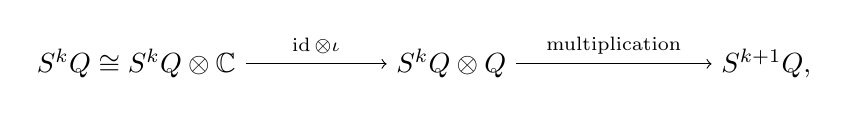
\begin{tikzpicture}[auto,baseline=(current  bounding  box.center)]
    \path[anchor=base] (0,0) node (1) {$S^kQ\cong S^kQ\otimes \bC$} +(4,0) node (2) {$S^kQ\otimes Q$} +(8,0) node (3) {$S^{k+1}Q$,};
    \draw[->] (1) to[bend left=0] node[pos=.5,auto] {$\scriptstyle \id\otimes\iota$} (2);
    \draw[->] (2) to[bend left=0] node[pos=.5,auto] {$\scriptstyle \text{multiplication}$} (3);
  \end{tikzpicture}
\end{equation}
where $\iota:\bC\to Q$ is the embedding defining $Q$ as an extension of $F$ by $\bC$. This gives rise to an exact sequence


\begin{equation}\label{eq:1}
  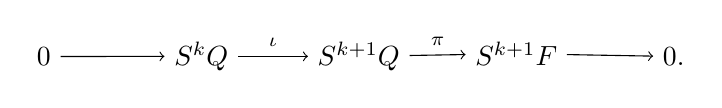
\begin{tikzpicture}[auto,baseline=(current  bounding  box.center)]
    \path[anchor=base] (0,0) node (01) {$0$} +(2,0) node (l) {$S^kQ$} +(4,0) node (m) {$S^{k+1}Q$} +(6,0) node (r) {$S^{k+1}F$} +(8,0) node (02) {$0$.};
    \draw[->] (01) to[bend left=0] node[pos=.5,auto] {$\scriptstyle $} (l);
    \draw[->] (l) to[bend left=0] node[pos=.5,auto] {$\scriptstyle \iota$} (m);
    \draw[->] (m) to[bend left=0] node[pos=.5,auto] {$\scriptstyle \pi$} (r);
    \draw[->] (r) to[bend left=0] node[pos=.5,auto] {$\scriptstyle $} (02);
  \end{tikzpicture}
  % 0\to S^nQ\to S^{n+1}Q\to S^{n+1}F\to 0.
\end{equation}

Taking the colimit (or simply union)
\begin{equation}\label{eq:12}
  I:=\varinjlim_k S^kQ,
\end{equation}
we obtain a $\fg$-module that has an infinite ascending filtration representable schematically as 

% % \[
% %   \tikz[anchor=base]{
% %     \path (0,0) node [minimum height=1cm] (0) [draw] {$\bC$} +(0,1) node [minimum height=1cm] (1) [draw] {$F$} +(0,2) node [minimum height=1cm] (3) [draw] {$S^2F$} +(0,3) node {$\vdots$};          
% %   }
% % \]
% %

\begin{equation}\label{eq:ifilt}
  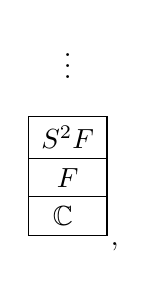
\begin{tikzpicture}[auto,baseline=(current  bounding  box.center)]
    \path (0,0) node[name=1, minimum width=1cm, rectangle split, rectangle split parts=3, draw, rectangle split draw splits=true, align=center] 
    { $S^2F$
      \nodepart{two} $F$
      \nodepart{three} $\bC$
    } + (0,1.5) node {$\vdots$};
	\path (0.6,-0.9) node {$,$};
    
    % \draw (1.text split west) -- (1.text split east);
  \end{tikzpicture}
\end{equation}
where the boxes indicate the layers (successive quotients) of the filtration.

% % We write $I_n$, $n\ge 0$ for the length-$(n+1)$ truncations of $I$ (so $I_0=\bC$, $I_1=Q$, etc.). It will also be convenient to set $I_{-1}=0$.

The morphism
\begin{equation}\label{eq:2}
  \psi: I\to I/\bC \to F\otimes I
\end{equation}
to be defined below will play a central role in the sequel; we will occasionally write $\psi$ for the resulting factorization $I/\bC\to F\otimes I$ as well, leaving it to context to separate the two possible meanings.

We obtain the morphism $\psi$ as a colimit $\varinjlim_k \psi^k$ where
\begin{equation}\label{eq:psik}
  \psi^k:S^{k}Q\to (S^{k}Q)/\bC \to F\otimes S^{k-1}Q.
\end{equation}
The latter map is defined as follows. First, recall that the symmetric algebra
\begin{equation*}
  S^{\bullet}Q = \bigoplus_{k\ge 0}S^kQ
\end{equation*}
has a graded Hopf algebra structure \cite[p.228]{Sweedler} making the degree-one elements {\it primitive}, i.e. such that the comultiplication
\begin{equation}\label{eq:delta}
  \Delta: S^{\bullet}Q\to S^{\bullet}Q\otimes S^{\bullet}Q
\end{equation}
is the unique algebra map defined by
\begin{equation*}
  S^{\bullet}Q\supset Q\ni v\mapsto v\otimes 1\oplus 1\otimes v\in (Q\otimes\bC)\oplus (\bC\otimes Q)\subset S^{\bullet}Q\otimes S^{\bullet}Q. 
\end{equation*}
The comultiplication \Cref{eq:delta} is a morphism of $\fg$-modules. By definition, the map \Cref{eq:psik} is given by

\begin{equation}\label{eq:3}
  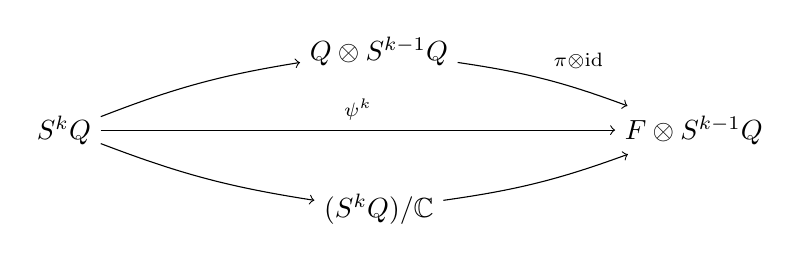
\begin{tikzpicture}[auto,baseline=(current  bounding  box.center)]
    \path[anchor=base] (0,0) node (1) {$S^{k}Q$}
    +(4,1) node (2) {$Q\otimes S^{k-1}Q$}
    +(8,0) node (3) {$F\otimes S^{k-1}Q$}
    +(4,-1) node (4) {($S^{k}Q)/\bC$};
    \draw[->] (1) to[bend left=6] node[pos=.5,auto] {$\scriptstyle $} (2);
    \draw[->] (2) to[bend left=6] node[pos=.5,auto] {$\scriptstyle \pi\otimes\id$} (3);
    \draw[->] (1) to[bend right=6] node[pos=.5,auto,swap] {$\scriptstyle $} (4);
    \draw[->] (4) to[bend right=6] node[pos=.5,auto,swap] {$\scriptstyle $} (3);
    \draw[->] (1) to[bend right=0] node[pos=.5,auto] {$\scriptstyle \psi^k$} (3);    
  \end{tikzpicture}
\end{equation}
where
\begin{itemize}
\item[$-$] the upper left{-}hand arrow is the $Q\otimes S^{k-1}Q$-component of the comultiplication
  \begin{equation*}
    \Delta:S^kQ\to \bigoplus_{i=0}^k S^iQ\otimes S^{k-i}Q
  \end{equation*}
  described above.
\item[$-$] $\pi$ is the epimorphism fitting in \Cref{eq:1}.
\end{itemize}

To make sense of $\varinjlim_k \psi^k$ we would have to argue that the maps $\psi^k$ are compatible with the embeddings
\begin{equation*}
  \iota:S^kQ\hookrightarrow S^{k+1}Q
\end{equation*}
in \Cref{eq:1}, i.e. that the diagrams
\begin{equation*}
 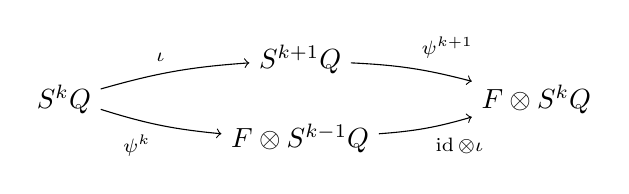
\begin{tikzpicture}[auto,baseline=(current  bounding  box.center)]
  \path[anchor=base] 
  (0,0) node (l) {$S^kQ$} 
  +(6,0) node (r) {$F\otimes S^{k}Q$}
  +(3,.5) node (u) {$S^{k+1}Q$}
  +(3,-.5) node (d) {$F\otimes S^{k-1}Q$}
  ;
  \draw[->] (l) to[bend left=6] node[pos=.5,auto] {$\scriptstyle \iota$} (u);
  \draw[->] (u) to[bend left=6] node[pos=.5,auto] {$\scriptstyle \psi^{k+1}$} (r);
  \draw[->] (l) to[bend right=6] node[pos=.5,auto,swap] {$\scriptstyle \psi^k$} (d);
  \draw[->] (d) to[bend right=6] node[pos=.5,auto,swap] {$\scriptstyle \id\otimes\iota$} (r);  
 \end{tikzpicture}
\end{equation*}
commute for arbitrary $k$. This can be seen by direct examination, fixing a basis $\{v_{\alpha}\}$ for $Q$ with a distinguished element $v_0=1\in \bC\subset Q$ and noting that the upper left{-}hand map in \Cref{eq:3} is defined on monomials by
\begin{equation}\label{eq:expldelta}
  v_{\alpha_1}\cdots v_{\alpha_k}\mapsto \sum_{i=1}^k v_{\alpha_i}\otimes v_{\alpha_1}\cdots v_{\alpha_{i-1}}v_{\alpha_{i+1}}\cdots v_{\alpha_k}. 
\end{equation}

% % The latter map is obtained as 
% % \begin{equation}\label{eq:3}
% %   \begin{tikzpicture}[auto,baseline=(current  bounding  box.center)]
% %     \path[anchor=base] (0,0) node (1) {$S^{k}Q$}
% %     +(3,1) node (new) {$Q^{\otimes k}$}
% %     +(6,1) node (2) {$Q\otimes S^{k-1}Q$}
% %     +(9,0) node (3) {$F\otimes S^{k-1}Q$}
% %     +(4.5,-1) node (4) {($S^{k}Q)/\bC$};
% %     \draw[->] (1) to[bend left=6] node[pos=.5,auto] {$\scriptstyle $} (new);
% %     \draw[->] (new) to[bend left=6] node[pos=.5,auto] {$\scriptstyle \id_Q\otimes \pi_{k-1}$} (2);
% %     \draw[->] (2) to[bend left=6] node[pos=.5,auto] {$\scriptstyle \pi\otimes\id$} (3);
% %     \draw[->] (1) to[bend right=6] node[pos=.5,auto,swap] {$\scriptstyle $} (4);
% %     \draw[->] (4) to[bend right=6] node[pos=.5,auto,swap] {$\scriptstyle $} (3);
% %     \draw[->] (1) to[bend right=0] node[pos=.5,auto] {$\scriptstyle \psi^m$} (3);    
% %   \end{tikzpicture}
% % \end{equation}
% % where
% % \begin{itemize}
% % \item the upper left hand arrow is the embedding of the image of the full symmetrization operator;
% % \item $\pi_{k-1}:Q^{\otimes (k-1)}\to S^{k-1}Q$ is the canonical surjection;
% % \item $\pi$ is the epimorphism fitting in \Cref{eq:1}.
% % \end{itemize}
% % 



\begin{lemma}\label{le.correct-ker}
  The kernel of $\psi:I\to F\otimes I$ is precisely $\bC$.
\end{lemma}
\begin{proof}
  The kernel of the upper right-hand map in \Cref{eq:3} is
  \begin{equation}\label{eq:ck-1}
   \mathbb{C}\otimes S^{k-1}Q\subset Q\otimes S^{k-1}Q,
  \end{equation}
  so we are in effect claiming that the preimage of \Cref{eq:ck-1} through the ``partial comultiplication''
  \begin{equation}\label{eq:partdelta}
    S^kQ\to Q\otimes S^{k-1}Q
  \end{equation}
  is $\bC\subset S^kQ$.

  This is easily seen from the explicit description \Cref{eq:expldelta} of the comultiplication \Cref{eq:partdelta}.
\end{proof}  


% %   intersection
% % \begin{equation*}
% %  \begin{tikzpicture}[auto,baseline=(current  bounding  box.center)]
% %   \path[anchor=base] (0,0) node (1) {$\bullet$} +(6,0) node (2) {$Q\otimes S^{k-1}Q$} +(3,.5) node (mu) {$\bC\otimes S^{k-1}Q$} +(3,-.5) node (md) {$S^{k}Q$};
% %   \draw[right hook ->] (1) to[bend left=6] node[pos=.5,auto] {$\scriptstyle $} (mu);
% %   \draw[right hook->] (mu) to[bend left=6] node[pos=.5,auto] {$\scriptstyle $} (2);
% %   \draw[right hook->] (1) to[bend right=6] node[pos=.5,auto] {$\scriptstyle $} (md);
% %   \draw[right hook->] (md) to[bend right=6] node[pos=.5,auto] {$\scriptstyle $} (2);    
% %  \end{tikzpicture}
% % \end{equation*}
% % is
% % \begin{equation*}
% %   \bC\cong \bC\otimes \bC\subset Q\otimes S^{k-1}Q;
% % \end{equation*}
% % the definition of the symmetrization operator makes this clear, however.
% % 


%%%%%%%%%%%%%%%%%%%%%%%%%%%%%%%%%%%%%%%%%%%%%%%%%%%%%%%%%%%%%%%%%%%%%%%%%%%%%
\subsection{Order}\label{subse:ord}

Following (or rather amplifying) \cite{us0}, we order the quadruples $(l,m,n,p)$ of non-negative integers by setting
\begin{equation*}
  (l,m,n,p)\preceq (l',m',n',p')
\end{equation*}
precisely if
\begin{align*}
  l\ge l',\quad m\le m',&\quad p\ge p',\quad n\le n' \numberthis \label{eq:ord}\\
 % m\le m'\quad&\text{and}\quad n\le n'\\
  l+m-n-p = \,\,& l'+m'-n'-p'.
\end{align*}

For a quadruple $s=(l,m,n,p)$ we define a family $\Sigma_s$ of morphisms
\begin{equation*}
  I_s=J_s\otimes I\to J_{s'}\otimes I=I_{s'}
\end{equation*}
for various $s'\prec s$ as follows:
\begin{itemize}
\item[$-$] first, those of the form $\theta\otimes\id_I$ where $\theta\in \Theta_s$ as in \cite[\S 3.2]{us0};
\item[$-$] secondly, $\id_{J_s}\otimes \psi_0$ where
  \begin{equation}\label{eq:16}
    \psi_0:I\to F\otimes I
  \end{equation}
  is the morphism in \Cref{eq:2}. 
\end{itemize}

The morphisms of the first type are such that their joint kernel is
\begin{equation*}
  L_{l,m,n,p}\otimes I\subseteq  J_{l,m,n,p}\otimes I=I_{l,m,n,p}. 
\end{equation*}
On the other hand, the kernel of $\psi_0$ is $\bC\subset I$ and hence the joint kernel of $\Sigma_s$ is
\begin{equation}\label{eq:4}
  L_{l,m,n,p}\cong L_{l,m,n,p}\otimes \bC\subset J_{l,m,n,p}\otimes I=I_{l,m,n,p}. 
\end{equation}

We now want to argue that \Cref{eq:4} is precisely the inclusion of the socle:

\begin{proposition}\label{pr.soc}
  For every choice of non-negative integers $l$, $m$, $n$, and $p$, the object $L_{l,m,n,p}$ is the socle of $I_{l,m,n,p}$ via the inclusion \Cref{eq:4}. 
\end{proposition}

This will require some preparation. First, we have the following remark, in the spirit of \cite[Lemma 3.1]{us0}. 

\begin{lemma}\label{le.tens-dense}
  Let $\fG$ be a Lie algebra and $I\subseteq \fG$ an ideal. Suppose $U\subseteq U'$ is an essential inclusion of $\fG/I$-modules and $D$ is a $\fG$-module on which $I$ acts densely. % and irreducibly with $\End_I(D)=\bK$. Then,
  Then the inclusion
  \begin{equation*}
    U\otimes D\subseteq U'\otimes D
  \end{equation*}
  is also essential.
\end{lemma}
\begin{proof}
  Let $w_1,~\ldots,~w_k$ be linearly independent vectors in $D$ ($k \ge 1$), and consider an element
  \begin{equation*}
    f:=\sum_{i=1}^k u_i\otimes w_i\in U'\otimes D
  \end{equation*}
  with non-zero $u_i$. We claim that for every $\overline{x}\in \fG/I$, there is $x\in \fG$ so that $\overline{x}$ is the image of $x$ and $$x f=\sum_i \overline{x}u_i\otimes w_i.$$
%  \begin{itemize}
%  \item[$-$]$x$ has image $\overline{x}$ modulo $I$;
%  \item[$-$]$x f=\sum_i \overline{x}u_i\otimes w_i$.   
%  \end{itemize}
  To see this, first choose an arbitrary $y\in \fG$ with image $\overline{x}$ in $\fG/${$I$}, so that
  \begin{equation*}
    y f = \sum_i \overline{x}u_i\otimes w_i + \sum_i u_i\otimes yw_i.
  \end{equation*}
  On the other hand, by the density assumption there is some $a\in I$ satisfying $aw_i=yw_i$ for all $i$, and we can simply set $x=y-a$.

  Having settled the claim and fixed an element $f$ as above, we can now proceed. The density of $U\subseteq U'$ means that we can find $\overline{a}$ in the universal enveloping algebra $U(\fG/I)$ such that
  \begin{itemize}
  \item[$-$] all $\overline{a}u_i$ belong to $U$, and
  \item[$-$] at least one of them ($\overline{a}u_j$, say) is non-zero.
  \end{itemize}
  Decomposing $\overline{a}$ as a polynomial in elements $\overline{x}\in \fG/I$ and lifting each of those to elements $x\in \fG$ as in the claim, we obtain an element $a\in U(\fG)$ with
  \begin{equation*}
    a f = \sum_i \overline{a}u_i\otimes w_i\in U\otimes D. 
  \end{equation*}
  Since $w_i$ are linearly independent and $\overline{a}u_j\ne 0$, this is a non-zero element of $U\otimes D$, and the proof is complete.
\end{proof}

% % 
% %   Let $u\otimes w\in U'\otimes D$ be a non-zero simple tensor. We claim that for every $\overline{x}\in \fG/I$, there is an $x\in \fG$ such that:
% %   \begin{itemize}
% %   \item[$-$]$x$ has image $\overline{x}$ modulo $I$;
% %   \item[$-$] $x(u\otimes w)=\overline{x}u\otimes w$.   
% %   \end{itemize}
% %   To see this, first choose an arbitrary $y\in \fG$ with image $\overline{x}$ in $\fG/${$I$}. We have
% %   \begin{equation*}
% %     y(u\otimes w) = \overline{x}u\otimes w + u\otimes yw.
% %   \end{equation*}
% %   On the other hand, by the density assumption there is some $a\in I$ such that $aw=yw$, and we can simply set $x=y-a$.
% % 
% %   Now let $w_1$ up to $w_k$ be linearly independent vectors in $D$ and consider an  element
% %   \begin{equation*}
% %     f:=\sum_{i=1}^k u_i\otimes w_i\in U'\otimes D.
% %   \end{equation*}
% % Using the fact that $U\subseteq U'$ is essential and the claim above, there is an element $x\in \fG$ such that 
% % \begin{equation}\label{eq:5}
% %   xf = \sum_{i=1}^k q_i\otimes w_i
% % \end{equation}
% % %where the $q_i$ entries are vectors with $q_1\in U'$.
% % with $q_1\in U$. We can now repeat the procedure, acting on the right-hand side of \Cref{eq:5} with another element $x'\in \fG$ so that the resulting sum is of the same form, with $q_1$ and $q_2$ in $U$. By recursion, we will eventually obtain an element of the form
% % \begin{equation*}
% %   \sum_i q_i\otimes w_i\in U\otimes D
% % \end{equation*}
% % in the $U(\fG)$-submodule of $U'\otimes D$ generated by $f$. This finishes the proof.
% % 


The following result will require some additional conventions and elaboration. Recall that $Q$ is the quotient
  \begin{equation*}
    V^*\otimes V^*_*/(\text{traceless tensors in }V^*\otimes V + V_* \otimes   V^*_*).
  \end{equation*}
  We noted above that we identify the space $ V^*\otimes V^*_*$ with finite-rank infinite $\mathbb{N}\times \mathbb{N}$-matrices, and hence the quotient consists of equivalence classes of such matrices, where two are declared equivalent whenever they differ by a traceless matrix $(a_{ij})$ such that $a_{ij}=0$ for large enough $i$ and $j$. %along at most finitely many rows or columns (and this is extended minimally to an equivalence relation).

We fix a basis $\{e_{\alpha}\}_{\alpha\in A}$ of $Q$ as follows: 

\begin{itemize}
\item[$-$] $e_0=1\in \bC$;
\item[$-$] all other basis elements are classes of rank-1 matrices of the form $v^* \otimes  v $ for $v^*\in V^*$ and   $v\in V^*_*$.   
\end{itemize}


\begin{lemma}\label{le.prscr-ann}
  Let $X\subset V_*^*-V$ and $X^*\in V^*-V_*$ be finite subsets, linearly independent modulo $V$ and respectively $V_*$. Fix $x_0\in X$ and $x_0^*\in X^*$. There is an element $g\in \fg$ such that
  \begin{itemize}
  \item[$-$] $gx\in V$ for all $x\in X$,   
  \item[$-$] $gx^*\in V_*$ for all $x^*\in X^*$,
  \item[$-$] $g(  x_0^* \otimes  x_0)$ has non-zero trace,
  \item[$-$] $g(x^*\otimes x )$ has zero trace for all other choices of $x\in X$ and $x^*\in X^*$.
  \end{itemize}
\end{lemma}
\begin{proof}
  The conclusion will follow from the remark that $\fg$ acts densely on sets $X\cup X^*$, i.e. that given $x\in X$ and $x^*\in X^*$, the vectors $gx\in V \text{ and }gx^* \in V_*$ can be prescribed arbitrarily. Keeping this in mind, we can then find $g\in \fg$ such that
  \begin{itemize}
  \item[$-$] $gx=0$ for all $x\in X$, 
  \item[$-$] $gx^*=0$ for all $x\in X^*\setminus\{x_0^*\}$, 
  \item[$-$] the inner product of $gx_0^*$ with every $x\in X\setminus\{x_0\}$ vanishes, 
  \item[$-$] the inner product of $gx_0^*$ with $x_0$ does not vanish.
  \end{itemize}
  This choice will meet the requirements of the statement, hence the conclusion.
\end{proof}


\begin{proposition}\label{pr.ann}
  Let $F\subset W\cup W_*$ be a finite set of vectors and
  \begin{equation*}
   \fK_{F}:=\mathrm{Ann}_{\fg}F\subset\fg 
  \end{equation*}
  be the Lie subalgebra that annihilates all elements of $F$. Then for every positive integer $k$ the inclusion
  \begin{equation*}
    \bC\subset S^kQ
  \end{equation*}
  is essential over $\fK=\fK_F$.
\end{proposition}
\begin{proof}
  We have to show that the $\fK$-submodule generated by any non-zero element of $S^kQ$ intersects $\bC$. We fix a basis $\{e_{\alpha}\}_{\alpha\in A}$ for $Q$ containing $e_0=1\in \bC$, as in the discussion preceding the statement of the present result. If we put a total order $\le $ on the index set $A$, the elements
  \begin{equation}\label{eq:10}
    e_{\bf t}=e_{\alpha_1}\cdots e_{\alpha_k}:=\sigma(e_{\alpha_1}\otimes \cdots\otimes e_{\alpha_k})
  \end{equation}
  for tuples
  \begin{equation*}
    {\bf t}=(\alpha_1,\cdots,\alpha_k),\ \alpha_1\le \cdots\le \alpha_k\in A
  \end{equation*}
  form a basis of $S^kQ$, where $\sigma$ denotes the symmetrization operator on $Q^{\otimes k}$.

  We assign $1=e_0$ degree zero and every other $e_{\alpha}$ degree $1$, thus allowing us to define a degree between $0$ and $k$ for each element \Cref{eq:10} and by extension for each $x\in S^kQ$, as the largest degree of a basis element \Cref{eq:10} appearing in a decomposition of $x$.

  We can now prove the claim that
  \begin{equation*}
    \bC\subseteq U(\fK)x
  \end{equation*}
  by induction on the degree of $x$. Since the base case $\deg(x)=0$ requires no proof, we focus on the induction step.

  Decompose
  \begin{equation}\label{eq:11}
    x=\sum c_{\bf t}e_{\bf t},\ c_{\bf t}\ne 0,
  \end{equation}
  with $\deg(x)>0$. By \Cref{le.prscr-ann} we can arrange for an element $g\in \fK$ such that
  \begin{itemize}
  \item[$-$] $g$ annihilates all elements of $F\subset W\cup W_*$,
  \item[$-$] $g$ sends one of the elements $1\ne e_{\alpha}$ appearing among the tensorands in \Cref{eq:11} to a non-zero scalar multiple of $e_0$,
  \item[$-$] $g$ annihilates all other $e_{\alpha}$ appearing in \Cref{eq:11}.
  \end{itemize}

  Clearly then
  \begin{equation*}
    \deg(gx) = \deg(x)-1,
  \end{equation*}
  and we can conclude the argument by using the induction hypothesis.
\end{proof}


% % 
% % We now need to make a detour for further notation and auxiliary results. Consider a family
% % \begin{equation*}
% %   D_f\subseteq E_f,\ f\in \cF
% % \end{equation*}
% % of inclusions in a tensor abelian category (the reader may as well assume these are modules over a Lie algebra). For a tuple
% % \begin{equation*}
% % {\bf f}= (f_1,\cdots,f_n)\subset \cF^n
% % \end{equation*}
% % we write
% % \begin{equation*}
% %   E_{\bf f}=E_{f_1}\otimes \cdots E_{f_n}. 
% % \end{equation*}
% % For any $f\in \cF$ and binary number $r\in\{0,1\}$ we set 
% % \begin{equation*}
% %   {}_rE_f=
% %   \begin{cases}
% %     D_f&\text{if }r=0\\
% %     E_f&\text{if }r=1
% %   \end{cases}
% % \end{equation*}
% % Now let
% % \begin{equation*}
% %   {\bf r}=(r_1,\cdots,r_n)\subset \{0,1\}^n
% % \end{equation*}
% % be a binary tuple and ${\bf f}=(f_1,\cdots,f_n)\in \cF^n$ as above. We denote
% % \begin{equation*}
% %   {}_{\bf r}E_{\bf f}:={}_{r_1}E_{f_1}\otimes\cdots\otimes {}_{r_n}E_{f_n}.
% % \end{equation*}
% % Note that $E:={}_{\bf r}E_{\bf f}$ has an increasing filtration 
% % \begin{equation*}
% %   0=E_{-1}\subseteq E_0\subseteq\cdots\subseteq E_n=E
% % \end{equation*}
% % where
% % \begin{equation*}
% %   E_t:=\sum_{|{\bf r}|=t}{}_{\bf r}E_{\bf f},\quad |{\bf r}|:=\sum_{i=1}^n r_i. 
% % \end{equation*}
% % 
% % Next, recall:
% % \begin{definition}
% %   An increasing filtration of an object $E$ in an abelian category by subobjects $E_{\alpha}$ for $\alpha\in (P,\le)$ ranging over a poset is {\it essential} if
% %   \begin{equation*}
% %     E_{\beta}/E_{\alpha}\subseteq E_{\gamma}/E_{\alpha}
% %   \end{equation*}
% %   is essential whenever $\alpha\le \beta\le \gamma$ in $(P,\le)$.
% % \end{definition}
% % 
% % 
% % 
% % 
% % 
% % We filter the object $V^{*\otimes n}\otimes V_*^{*\otimes p}$ as follows.
% % 
% % Let ${\bf r}=(r_1,\cdots,r_n)$ and ${\bf s}=(s_1,\cdots, s_p)$ be binary tuples (i.e. $r_i$ and $s_j$ are $0$ or $1$). We write
% % \begin{equation*}
% %   V^*_r=
% %   \begin{cases}
% %     V^*&\text{if }r=1\\
% %     V_*&\text{if }r=0
% %   \end{cases}
% % \end{equation*}
% % and similarly,
% % \begin{equation*}
% %   V^*_{*r}=
% %   \begin{cases}
% %     V_*^*&\text{if }r=1\\
% %     V&\text{if }r=0
% %   \end{cases}  
% % \end{equation*}
% % Now set
% % \begin{equation*}
% %   V^{*\otimes{\bf r}} = V^*_{r_1}\otimes\cdots\otimes V^*_{r_n}
% % \end{equation*}
% % and similarly for $V^*_*$. 
% % 
% % The {\it weight} $|{\bf r}|$ of a binary vector is the number of entries equal to $1$ (or in other words, the sum of the entries, regarded as integers).
% % 
% % Write
% % \begin{equation*}
% %   D=D^{n,p}:=V^{*\otimes n}\otimes V_*^{*\otimes p}
% % \end{equation*}
% % and, for $0\le x\le n$ and $0\le y\le p$ set
% % \begin{equation*}
% %   D_{x,y}=D^{n,p}_{x,y} := \sum_{|{\bf r}|=x,|{\bf s}|=y}V^{*\otimes {\bf r}}\otimes V_*^{*\otimes {\bf s}}.
% % \end{equation*}
% % Clearly,
% % \begin{equation*}
% %   D_{x,y}\subseteq D_{x',y'} 
% % \end{equation*}
% % whenever
% % \begin{equation}\label{eq:8}
% %   x\le x'\quad\text{and}\quad y\le y',
% % \end{equation}
% % so this provides an increasing filtration of the object $D$ by the objects $D_{x,y}$, indexed by the poset of pairs $(x,y)$ ordered via \Cref{eq:8}.
% % 
% % 
% % 
% % The following result is a ``two-sided'' version of \cite[Proposition 2]{Chi14}.
% % 
% % \begin{proposition}\label{pr.ess-filt}
% %   The filtration of the object $D=D^{n,p}$ provided by the $D_{x,y}$ is essential.
% % \end{proposition}
% % \begin{proof}
% % 
% %   
% %   
% % \end{proof}
% %

\pf{pr.soc}
\begin{pr.soc}
  We know that $L_{l,m,n,p}$ is semisimple by \cite[Corollary 4.3]{us0}, so it suffices to show that \Cref{eq:4} is essential. 

  Since $W$, $W_*$ and $I$ are trivial as $\fsl(\infty)$-modules and
  \begin{equation*}
    V_{m,n}\subset V^{*\otimes m}\otimes V^{\otimes n}
  \end{equation*}
  is the socle over $\fsl(\infty)$, it follows by restricting to the latter subalgebra of $\fg$ that the inclusion
  \begin{equation*}
    L_{l,m,n,p}\otimes I\subset J_{l,m,n,p}\otimes I
  \end{equation*}
  is essential, reducing the goal to proving that so is the inclusion
  \begin{equation}\label{eq:6}
    L_{l,m,n,p}\subset L_{l,m,n,p}\otimes I. 
  \end{equation}
  We can simplify this further: recall that
  \begin{equation*}
    L_{l,m,n,p}=W_*^{\otimes l}\otimes V_{m,n}\otimes W^{\otimes p}.
  \end{equation*}
  Now apply \Cref{le.tens-dense} in the following setup:
  \begin{itemize}
  \item[$-$] $\fG=\fg$ and $I=\fsl(\infty)$;
  \item[$-$] the inclusion $U\subseteq U'$ is
    \begin{equation}\label{eq:7}
      W_*^{\otimes l}\otimes W^{\otimes p}\subset W_*^{\otimes l}\otimes W^{\otimes p}\otimes I;
    \end{equation}
  \item[$-$] $D$ is any of the simple direct summands $V_{\mu,\nu}$ of $V_{m,n}$.    
  \end{itemize}
  \Cref{le.tens-dense} then shows that the inclusion \Cref{eq:6} is indeed %dense 
  essential, provided the inclusion \Cref{eq:7} is. In other words, it is enough to consider $m=n=0$ in \Cref{eq:6}. Since $I$ is the union of $S^kQ$ as $k\to \infty$, it will furthermore be sufficient to argue that, for every $l$, $p$ and $k$, the inclusion
  \begin{equation}\label{eq:9}
    W_*^{\otimes l}\otimes W^{\otimes p}\subset W_*^{\otimes l}\otimes W^{\otimes p}\otimes S^kQ
  \end{equation}
  is essential.

  We can now conclude via \Cref{pr.ann}: an arbitrary non-zero element of the right-hand side of \Cref{eq:9} is of the form
  \begin{equation*}
    \sum_{i=1}^r e_i\otimes v_i
  \end{equation*}
  where $e_i=\sum_{j} a_{i,j} \otimes b_{i,j}$ are linearly independent elements of $W_*^{\otimes l}\otimes W^{\otimes p}$ and $v_i\in S^kQ$. Now let $F\subset W\cup W_*$ be the finite set of vectors $\{a_{i,j}, b_{i,j}\}$ and consider the annihilator $\fK_F$ of $F$, as in \Cref{pr.ann}.

  The Lie algebra $\fK_F$ leaves the subspace
  \begin{equation*}
    \left(\bigoplus_{i=1}^r \bC e_i \right)\otimes S^kQ
  \end{equation*}
  invariant and its action makes that space isomorphic to $(S^kQ)^{\oplus r}$. The conclusion thus follows from \Cref{pr.ann}.
\end{pr.soc}


%%%%%%%%%%%%%%%%%%%%%%%%%%%%%%%%%%%%%%%%%%%%%%%%%%%%%%%%%%%%%%%%%%%%%%%%%%%%%
\subsection{Simple objects and their endomorphism algebras}\label{subse:endo}

The main result of the present subsection is the following (presumably expected) claim.

\begin{theorem}\label{th:scalaralgs}
The simple objects $L_{\lambda,\mu,\nu,\pi}$ are mutually non-isomorphic and have scalar endomorphism algebras.   
\end{theorem}

The arguments, which require some groundwork, will be in the spirit of those used in the proof of the analogous statement \cite[Theorem 3.5]{us0}. First, recall \cite[Lemma 3.1]{us0}:



\begin{lemma}\label{le:dense-us0}
  Let $\fG$ be a Lie algebra and $J\subseteq \fG$ be an ideal. Suppose $U$, $U'$ are two $\fG/J$-modules and $D$ a $\fG$-module on which $J$ acts densely and irreducibly with $\End_J D=\bC$. Then, the inclusion
  \begin{equation*}
    \Hom_{\fG}(U,U')\ni f\mapsto f\otimes \id\in \Hom_{\fG}(U\otimes D,U'\otimes D)
  \end{equation*}
  is an isomorphism.
  \qedhere
\end{lemma}

\begin{proposition}\label{pr:gpendoalgs}
  For any two non-negative integers $l$, $p$ and Young diagrams $\mu$, $\nu$ the endomorphism algebra in $\bT$ of the object $W_{*l}\otimes V_{\mu,\nu}\otimes W_{p}$ is the group algebra $\bC [S_l\times S_p]$, with the two symmetric-group factors acting on the two outer tensorands. 
\end{proposition}
\begin{proof}
  We apply \Cref{le:dense-us0} to the ideal
  \begin{equation*}
    \fsl(\infty)=:J\subset \fG:=\fg,
  \end{equation*}
  with
  \begin{equation*}
    U=U'=W_{*l}\otimes W_p\quad\text{and}\quad D=V_{\mu,\nu}. 
  \end{equation*}
  The density of the action of $\fsl(\infty)$ on $V_{\mu,\nu}$ and the isomorphism $\End_{\fsl(\infty)} V_{\mu,\nu}\cong \bC$ follow by realizing the object $V_{\mu,\nu}$ as a colimit of irreducible $\fsl_n$-modules, while establishing an isomorphism
  \begin{equation*}
    \End_{\fg} ( W_{*l}\otimes W_p)\cong \bC[S_l\times S_p]
  \end{equation*}
  is entirely parallel to \cite[Proposition 3.2]{us0}, whose proof we do not reprise here. \Cref{le:dense-us0} then implies the desired isomorphism
  \begin{equation*}
    \End_{\fg} (W_{*l}\otimes V_{\mu,\nu}\otimes W_p)\cong  \End_{\fg} (W_{*l}\otimes W_p)\cong \bC[S_l\times S_p].
  \end{equation*}
\end{proof}


\pf{th:scalaralgs}
\begin{th:scalaralgs}
  According to \Cref{pr:gpendoalgs}, the endomorphism algebra
  \begin{equation}\label{eq:endss}
    \End_{\fg} (W_{*l}\otimes V_{\mu,\nu}\otimes W_{p})\cong \bC[S_l\times S_p]\cong \bC [S_l ]\otimes \bC [S_p]
  \end{equation}
  is semisimple. Since the tensor products
    $c_{\lambda}\otimes c_{\pi}\in \bC [S_l]\otimes \bC [S_p ]$
  of Young projectors ranging over diagrams with $|\lambda|=l,~|\pi|=p$,  
  form a complete system of equivalence classes of minimal idempotents in \Cref{eq:endss} under inner conjugation, the semisimple object $W_{*l}\otimes V_{\mu,\nu}\otimes W_{p}$ has simple constituents isomorphic to
  \begin{equation*}
    (c_\lambda\otimes c_{\pi})\left(W_{*l}\otimes V_{\mu,\nu}\otimes W_{p}\right) \cong L_{\lambda,\mu,\nu,\pi},
  \end{equation*}
  with  $L_{\lambda,\mu,\nu,\pi}$ not isomorphic to $ L_{\lambda',\mu,\nu,\pi'}$ for distinct pairs $(\lambda,\pi)\ne (\lambda',\pi')$ because
  \begin{equation*}
    c_{\lambda}\otimes c_{\pi}\text{ is not inner-conjugate to }c_{\lambda'}\otimes c_{\pi'}.
  \end{equation*}
  
  Furthermore, using Proposition \ref{pr:gpendoalgs}, we calculate 
  \begin{align*}
  \End_{\fg}L_{\lambda,\mu,\nu,\pi}&\cong \End_{\fg}\left((c_\lambda\otimes c_{\pi})\left(W_{*l}\otimes V_{\mu,\nu}\otimes W_{p}\right) \right)\\
  &\cong (c_\lambda\otimes c_{\pi})\End_{\fg}\left(W_{*l}\otimes V_{\mu,\nu}\otimes W_{p}\right)(c_\lambda\otimes c_{\pi})\\
  &\cong (c_\lambda\otimes c_{\pi})\bC[S_l\times S_p](c_\lambda\otimes c_{\pi}).
  \end{align*}
  Since $(c_{\lambda}\otimes c_{\pi})\bC[S_l\times S_p]=X$ is a simple $\bC[S_l\times S_p] $-module, we have $(c_{\lambda}\otimes c_{\pi})\bC[S_l\times S_p](c_{\lambda}\otimes c_{\pi})=\End_{\bC[S_l\times S_p]} X=\bC$, and the statement is proved.
  

\end{th:scalaralgs}


	


%%%%%%%%%%%%%%%%%%%%%%%%%%%%%%%%%%%%%%%%%%%%%%%%%%%%%%%%%%%%%%%%%%%%%%%%%%%%%
\subsection{The category $\bT$}\label{subse:ord-cat}

\begin{definition}\label{def:t}
  The category $\bT$ is the smallest full %monoidal symmetric 
  tensor Grothendieck subcategory of the category ${}_{\fg}\md$ of $\fg$-modules, closed under taking subquotients, and containing
  \begin{itemize}
  \item[$-$] the objects $V^*$ and $V_*^*$ (and hence also $J_s$ of \Cref{eq:j} for quadruples $s=(l,m,n,p)$);
  \item[$-$] the object $I$ of \Cref{eq:12}. 
  \end{itemize}
% % We denote by $\overline{\bT}$ the Grothendieck closure of $\bT$ in ${}_{\fg}\md$.   
\end{definition}

The indices $s=(l,m,n,p)$ form a poset $(\cP,\preceq)$ under the ordering introduced in \Cref{subse:ord}. Keeping that in mind, we have

\begin{proposition}\label{pr.is-ordered}
$\bT$ is an ordered Grothendieck category in the sense of \Cref{def.ord-gr}.   
\end{proposition}
\begin{proof}
  We have to check the conditions listed in \Cref{def.ord-gr}. Here, the objects $X_s$ will be the objects $I_s$ from \Cref{eq:13} for $s=(l,m,n,p)$.

  {Condition \emph{(\labelcref{item:3})}.} This follows from the fact that all $I_s$ have countable filtrations whose subquotients are simple objects of the form $L_{\lambda,\mu,\nu,\pi}$ as in \Cref{eq:s}. The latter is clear as the objects $J_s$ have finite length and $I$ has the filtration \Cref{eq:12}.
  %simply tensor the finite-length $J_s$ with the filtration of $I$ given by \Cref{eq:12}. 

% %   \vspace{.5cm}
% % 
% %   {\bf Condition \labelcref{item:4}.} Let $\cS\subset \cP$ be a non-empty totally ordered subset consisting of elements
% %   \begin{equation*}
% %     \cS\ni s = (l_s,m_s,n_s,p_s). 
% %   \end{equation*}
% %   

  {Condition \emph{(\labelcref{item:5})}.} This holds essentially by construction. 

  {Condition \emph{(\labelcref{item:6})}} is a consequence of \cite[Proposition 4.4]{us0}.  

  {Condition \emph{(\labelcref{item:7})}.} Once more, we filter $I_s=J_s\otimes I$ by first refining the socle filtration maximally of $J_s$ and then tensor by some maximal refinement of the filtration \Cref{eq:12}. %(maximally again, so all subquotients of the latter are simple).

  The successive subquotients
  \begin{equation*}
    S^{k+1}Q/S^kQ \cong S^{k+1}F= S^{k+1}(W\otimes W_*)
  \end{equation*}
  of \Cref{eq:12} can be decomposed as sums of objects of the form $W_{\lambda}\otimes W_{*\lambda}$ by part \emph{(\labelcref{item:1})} of \Cref{pr.plth}. Hence, tensoring a simple subquotient $S$
  of $J_s$ for some $s=(l,m,n,p)$ by such an object has the effect of increasing $l$ and $p$ by the same amount, thus resulting in some $t\prec s$ according to our ordering \Cref{eq:ord}.

  It thus remains to argue for simple subquotients of
  \begin{equation*}
    J_s=J_{l,m,n,p}=W_*^{\otimes l}\otimes V^{*\otimes m}\otimes V_*^{*\otimes n}\otimes W^{\otimes p}
  \end{equation*}
  instead. In this case though the filtration of $J_s$ is obtained either by surjecting one of the tensorands $V^*$ onto $W_*=V^*/V_*$ or similarly, one of the tensorands $V_*^*$ onto $W$, or by evaluating some $V^{*}$(respectively, $ V_{*}^{*} $) against some $V$(respectively, $ V_{*} $).

  All of these procedures map into $J_t$ for $t\prec s$, hence the conclusion.

  {Condition \emph{(\labelcref{item:8})}.} Indeed, for $s=(l,m,n,p)$ the object $I_s$ decomposes as
  \begin{equation*}
    I_s = \bigoplus_{\lambda,\mu,\nu,\pi}I_{\lambda,\mu,\nu,\pi}
  \end{equation*}
  where the sum ranges over $|\lambda|=l$, $|\mu|=m$, etc. The summands have simple respective socles $L_{\lambda,\mu,\nu,\pi}$ by \Cref{pr.soc}. 

  {Condition \emph{(\labelcref{item:9})}.} The morphisms $I_s\to I_t$ will be compositions of the obvious ones:
  \begin{itemize}
  \item[$-$] projecting one of the tensorands $V^*$ of $I_s=J_s\otimes I$ onto $W_*$;
  \item[$-$] the dual analogue, $V^*_*\to W$;
  \item[$-$] the surjection defining $Q$,%``partial pairing''
    \begin{equation}\label{eq:partpair}
      V^*\otimes V^*_*\to Q\subset I;
    \end{equation}
  \item[$-$] applying the morphism $I\to F\otimes I$ in \Cref{eq:16} to the tensorand $I$ of $I_s$. 
  \end{itemize}
  The verification that the joint kernel of these maps is as claimed is routine.  
\end{proof}

In particular, \cite[Proposition 2.5]{us1} and \Cref{pr.soc} together prove

\begin{theorem}\label{thm:hulls}
  For every quadruple $(\lambda,\mu,\nu,\pi)$ of Young diagrams, $I_{\lambda,\mu,\nu,\pi}$ is an injective hull in $\mathbb{T}$ of $L_{\lambda,\mu,\nu,\pi}$.
\end{theorem}

We record the following observation.

\begin{lemma}\label{le.defct}
  Let $i=(l,m,n,p)$ and $i'=(l',m',n',p')$ be two elements of the poset described in \Cref{eq:ord}. Then $i\preceq i'$ implies
  \begin{equation*}
    d(i,i') = l-l' + n'-n.
  \end{equation*}
\end{lemma}


\begin{remark}\label{re.symmetry}
  The category $\bT$ is symmetric with respect to the simultaneous interchange $V \leftrightarrow V_*$, $V^*\leftrightarrow V_*^*$. Numerically, this corresponds to $l\leftrightarrow p$ and $n\leftrightarrow m$. \Cref{le.defct} is compatible with this transformation: according to the last condition in \Cref{eq:ord} we have
  \begin{equation*}
    l-l' + n'-n = p-p' + m'-m,
  \end{equation*}
  so we could have substituted $p-p' + m'-m$  %the latter expression 
  for %the former 
  $l-l' + n'-n$ in \Cref{le.defct}. 
\end{remark}

%%%%%%%%%%%%%%%%%%%%%%%%%%%%%%%%%%%%%%%%%%%%%%%%%%%%%%%%%%%%%%%%%%%%%%%%%%%%%
\subsection{Injective resolutions}


We will now show that $\bC$ admits an injective resolution in $\bT$
\begin{equation}\label{eq:15}
  0\to \bC\to I_0\to I_1\to \cdots
\end{equation}
with %of $\bC$ in $\bT$. It turns out that
\begin{equation*}
  I_j\cong \Lambda^j F\otimes I. 
\end{equation*}
We will also see that $I_j/\mathrm{Im}(I_{j-1})$ admits an ascending filtration with layers
\begin{equation*}
  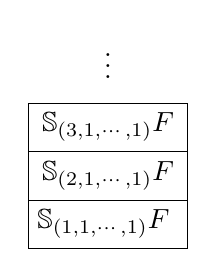
\begin{tikzpicture}
    \path (0,0) node[name=1, minimum width=1cm, rectangle split, rectangle split parts=3, draw, rectangle split draw splits=true, align=center] 
    { $\mathbb{S}_{(3,1,\cdots,1)}F$
      \nodepart{two} $\mathbb{S}_{(2,1,\cdots,1)}F$
      \nodepart{three} $\mathbb{S}_{(1,1,\cdots,1)}F$
    } + (0,1.5) node {$\vdots$};
    
    % \draw (1.text split west) -- (1.text split east);
  \end{tikzpicture}  
\end{equation*}
where each diagram has $j+1$ rows. 


To streamline the notation, for such Young diagrams we denote by $(l,j\times 1)$ the diagram with a row of length $l$ and $j$ single-box rows.

% a row count of $j$ in a diagram by a $j\times$ prefix; so $(2,j\times 1)$, for instance, is the $(j+1)$-row diagram with a row of length $2$ .  

To define the maps
\begin{equation}\label{eq:psij}
  \psi_j:\Lambda^j F\otimes I\to \Lambda^{j+1} F\otimes I
\end{equation}
we mimic the procedure used in the definition of \Cref{eq:16}. In fact, that notation will be compatible with \Cref{eq:psij}, in that we will recover that earlier map by setting $j=0$ in the latter. As before, \Cref{eq:psij} will be a colimit as $k\to \infty$ of maps
\begin{equation}\label{eq:psijk}
  \psi^k_j:\Lambda^j F\otimes S^kQ\to \Lambda^{j+1} F\otimes S^{k-1}Q.
\end{equation}

The analogue of diagram \Cref{eq:3} in this context is
\begin{equation}\label{eq:17}
  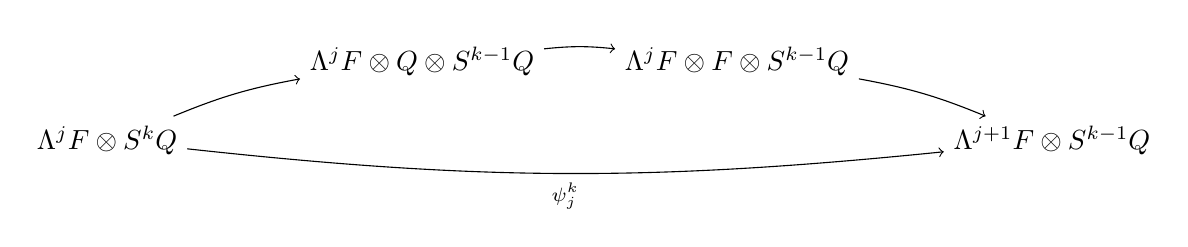
\begin{tikzpicture}[auto,baseline=(current  bounding  box.center)]
    \path[anchor=base] (0,0) node (1) {$\Lambda^j F\otimes S^{k}Q$}
    +(4,1) node (2) {$\Lambda^jF\otimes Q\otimes S^{k-1}Q$}
    +(8,1) node (3) {$\Lambda^jF\otimes F\otimes S^{k-1}Q$}
    +(12,0) node (4) {$\Lambda^{j+1}F\otimes S^{k-1}Q$};
    \draw[->] (1) to[bend left=6] node[pos=.5,auto] {$\scriptstyle $} (2);
    \draw[->] (2) to[bend left=6] node[pos=.5,auto] {$\scriptstyle $} (3);
    \draw[->] (1) to[bend right=6] node[pos=.5,auto,swap] {$\scriptstyle \psi_j^k$} (4);
    \draw[->] (3) to[bend left=6] node[pos=.5,auto] {$\scriptstyle $} (4);
  \end{tikzpicture}
\end{equation}
where
\begin{itemize}
\item[$-$] the upper left-hand map is $\id_{\Lambda^jF}\otimes \Delta$ with
  \begin{equation*}
    \Delta:S^kQ\to Q\otimes S^{k-1}Q,
  \end{equation*}
  the partial comultiplication also appearing in \Cref{eq:3};
\item[$-$] the upper middle map is $\id\otimes\pi\otimes \id$, with $\pi:Q\to F$ the canonical surjection (again as in \Cref{eq:3});
\item[$-$] the upper right-hand map is the multiplication
  \begin{equation*}
    \Lambda^j F\otimes F\to \Lambda^{j+1}F
  \end{equation*}
  in the exterior algebra $\Lambda^{\bullet} F$, tensored with the identity on $S^{k-1}Q$. 
\end{itemize}


To show that the maps \Cref{eq:psij} fit into a resolution \Cref{eq:15}, we begin with the following simple observation.

\begin{lemma}\label{le:jrows}
  Let $j,k$ be two positive integers and $X$ be a vector space of dimension larger than $j+1$. The map
\begin{equation}\label{eq:xmap}
  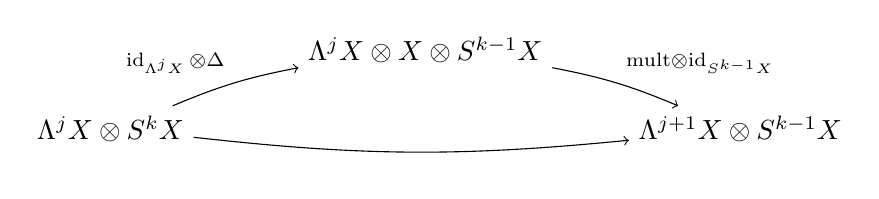
\begin{tikzpicture}[auto,baseline=(current  bounding  box.center)]
    \path[anchor=base] (0,0) node (1) {$\Lambda^j X\otimes S^{k}X$}
    +(4,1) node (2) {$\Lambda^jX\otimes X\otimes S^{k-1}X$}
    +(8,0) node (4) {$\Lambda^{j+1}X\otimes S^{k-1}X$};
    \draw[->] (1) to[bend left=6] node[pos=.5,auto] {$\scriptstyle \id_{\Lambda^j X}\otimes \Delta$} (2);
    \draw[->] (1) to[bend right=6] node[pos=.5,auto,swap] {$\scriptstyle $} (4);
    \draw[->] (2) to[bend left=6] node[pos=.5,auto] {$\scriptstyle \mathrm{mult}\otimes\id_{S^{k-1}X}$} (4);
  \end{tikzpicture}
\end{equation}
with $\Delta:S^k X\to X\otimes S^{k-1}X$ defined as in \Cref{eq:expldelta} annihilates the direct summand $\bS_{(k+1, (j-1)\times 1)} X$
 of $\Lambda^j X\otimes S^{k}X$ and maps the complementary summand  $\bS_{(k, j\times 1)} X$
of $\Lambda^j X\otimes S^{k}X$ isomorphically onto the corresponding summand of the codomain $\Lambda^{j+1} X\otimes S^{k-1}X${.}
\end{lemma}
\begin{proof}
  That the domain and codomain decompose as
  \begin{equation*}
    \Lambda^j X\otimes S^{k}X\cong \bS_{(k+1, (j-1)\times 1)}X \oplus \bS_{(k, j\times 1)}X
  \end{equation*}
  and
  \begin{equation*}
    \Lambda^{j+1} X\otimes S^{k-1}X\cong \bS_{(k, j\times 1)}X \oplus \bS_{(k-1, (j+1)\times 1)}X
  \end{equation*}
  respectively, follows from the Littlewood-Richardson rule \cite[Appendix A, (A.8)]{fh-bk}. The claim can be checked on finite-dimensional vector spaces first, where all four direct summands are irreducible representations of the algebraic group $GL(X)$, then passing to arbitrary $X$ by taking a colimit.
\end{proof}

Now consider one of the objects $\Lambda^j F\otimes I$, $j\ge 0$ under discussion. Since $I$ has the filtration \Cref{eq:ifilt}, %with consecutive quotients $S^k F$ for $k\ge 0$,
 the object $\Lambda^j F\otimes I$ has a filtration by the subobjects $\Lambda^{j} F\otimes S^{k}Q$, with consecutive quotients $\Lambda^j F\otimes S^k F$. Moreover, these quotients are decomposed as %the Littlewood-Richardson rule for tensoring two Schur functors we have, as noted in the proof of \Cref{le:jrows}, the decompositions
\begin{alignat*}{3}
  \Lambda^j F\otimes S^k F&\quad\cong\quad \bS_{(k+1, (j-1)\times 1)}F \quad \oplus\quad &&\bS_{(k, j\times 1)}F&&\quad \text{ for }j,k>0\\
  S^k F &\quad\cong\quad &&\bS_{(k)}F &&\quad \text{ for }j=0,\ k>0\numberthis\label{eq:decs}\\
  \Lambda^j F &\quad\cong\quad \bS_{(1,\ldots, 1)}F&& &&\quad \text{ for }k=0.
\end{alignat*}
%for the resulting subquotients of $\Lambda^j F\otimes I$ obtained by tensoring the exterior power by the original filtration \Cref{eq:ifilt} of $I$. In other words, each subquotient has a $j$-row summand (possibly zero, when $j=0$ and $k>0$) and a $(j+1)$-row summand (possibly zero, when $k=0$). 
Moreover, these decompositions are canonical, i.e. the summands are unique. 

We write
\begin{equation}\label{eq:kj}
  K_j:=\ker\left(\psi_j:\Lambda^j F\otimes I \to \Lambda^{j+1} F\otimes I\right)
\end{equation}
for the kernel of the map \Cref{eq:psij} and
\begin{equation*}
  K_j^k:= K_j\cap \left(\Lambda^j F\otimes S^kQ\right) = \ker\left(\psi_j:\Lambda^j F\otimes S^kQ \to \Lambda^{j+1} F\otimes S^{k-1}Q\right);
\end{equation*}
by convention, we set $K_j^{-1}=\{0\}$. We now have

\begin{lemma}\label{le:ksubq}
  For each $k\ge 0$ the quotient
  \begin{equation}\label{eq:kfq}
    K_j^k/K_j^{k-1}\subset \Lambda^j F\otimes \left(S^kQ/S^{k-1}Q\right)\cong \Lambda^j F\otimes S^k F
  \end{equation}
  is the $j$-row summand of $\Lambda^{j} F\otimes S^{k}F$. 
\end{lemma}
\begin{proof}
  The map $\psi_j$ respects the filtrations of its domain and codomain, by
  \begin{equation}\label{eq:filtrations}
    \Lambda^j F\otimes S^k Q\quad\text{and}\quad \Lambda^{j+1} F\otimes S^{k-1} Q
  \end{equation}
  respectively, and the associated graded map $\mathrm{gr}~\psi_j$, in degree $k$, is precisely \Cref{eq:xmap} with $X=F$. By \Cref{le:jrows} this means that the degree-$k$ kernel of $\mathrm{gr}~\psi_j$ is the $j$-row summand of $\Lambda^j F\otimes S^k F$. This verifies the statement at the associated-graded level.

  To conclude, it will suffice to construct gradings on the domain and codomain of $\psi_j$, compatible with $\psi_j$, that give back the filtrations by \Cref{eq:filtrations}. This would then prove that the filtered map $\psi_j$ arises from a grading, and hence that its kernel is the direct sum of the kernels of its homogeneous components. 

  We construct the requisite gradings as follows: as in the discussion preceding \Cref{le.correct-ker}, we fix a basis $\{v_{\alpha}\}$ for $Q$ with $v_0=1\in \bC\subset Q$, and assign
  \begin{equation*}
    \deg v_{\alpha}=
    \begin{cases}
      0&\text{for }\alpha=0\\
      1&\text{otherwise}.
    \end{cases}
  \end{equation*}
  One checks easily that $\psi_j$ preserves degrees, finishing the proof as described above.
\end{proof}

We can now finally complete the discussion on the injective resolution \Cref{eq:15}.

\begin{theorem}\label{th:injresc}
  The morphisms \Cref{eq:psij} fit into an exact sequence \Cref{eq:15}. 
\end{theorem}
\begin{proof}
  The maps $\psi_j$ fit into a sequence 
  \begin{equation}\label{eq:targetseq}
    0\to \bC\to I\stackrel{\psi_0}{\longrightarrow} F\otimes I\stackrel{\psi_1}{\longrightarrow} \Lambda^2 F\otimes I\stackrel{\psi_2}{\longrightarrow} \cdots
  \end{equation}
  (not yet known to be exact) of filtered vector spaces. \Cref{le:jrows} applied to $X=F$ shows that the associated graded sequence is exact, and the conclusion follows from the fact that, as seen in the proof of \Cref{le:ksubq}, the filtrations on the terms of \Cref{eq:targetseq} arise from gradings compatible with the maps $\psi_j$. 
\end{proof}

  
% % \Cref{le:ksubq} shows that the kernel \Cref{eq:kj} is the unique subobject of $\Lambda^j F\otimes I$ whose subquotients with respect to the filtration by $\Lambda^j F\otimes S^k Q$ consists precisely of the $j$-row summands of $\Lambda^j F\otimes S^k F$ (uniqueness follows from the fact that the decompositions \Cref{eq:decs} are canonical). 
% % 
% % But this means that 
% %
  

\begin{corollary}\label{cor.c}
For a simple object $X$ of $\bT$ we have  
%$$\operatorname{Ext}^{j}(X,\bC)=\{^{0} if X is not isomorphic to S_{X_\lambda,\emptyset,\emptyset}$$ 

\begin{equation*}
\operatorname{Ext}_{\bT}^{j}(X,\bC)=
 \begin{cases}
  0& \textup{ if } X \not\simeq  L_{\lambda,\emptyset,\emptyset,{\lambda^\perp}} \textup{ for }\lambda \textup{ with } |\lambda|=j\\
   %1250 &\text{se $\omega \in A^c$}
\mathbb{C}& \textup{ if } X \simeq  L_{\lambda,\emptyset,\emptyset,{\lambda^\perp}}  \textup{ for }\lambda \textup{ with } |\lambda|=j.


 \end{cases}
\end{equation*}
\end{corollary}
\begin{proof}
  The statement follows from the existence of the injective resolution \Cref{eq:15} of the trivial object $\bC$, since by \Cref{thm:hulls}  \begin{equation*}
  \mathrm{soc}I_j=\mathrm{soc}(\Lambda^j F\otimes I)=\Lambda^j F = \Lambda^j(W_*\otimes W),
  \end{equation*}
 which in turn, by \Cref{pr.plth}, \Cref{item:2}, decomposes as
   \begin{equation*}
  \bigoplus_{|\lambda|=j}W_{*\lambda}\otimes W_{\lambda^{\perp}}. 
  \end{equation*}
  
  %According to \Cref{th:injresc} we have an injective resolution \Cref{eq:15} for the trivial object $\bC$, whose $j^{th}$ term is
  %\begin{equation*}
  %  I_j:=\Lambda^j F\otimes I. 
  %\end{equation*}
  %By \Cref{thm:hulls} the socle of this object is
  %\begin{equation*}
  %  \Lambda^j F = \Lambda^j(W_*\otimes W), 
  %\end{equation*}
  %which in turn, by \Cref{pr.plth}, %\Cref{item:2}, decomposes as
 % \begin{equation*}
   % \bigoplus_{|\lambda|=j}W_{*\lambda}\otimes %W_{\lambda^{\perp}}. 
  %\end{equation*}
\end{proof}

%%%%%%%%%%%%%%%%%%%%%%%%%%%%%%%%%%%%%%%%%%%%%%%%%%%%%%%%%%%%%%%%%%%%%%%%%%%%%
\subsection{Koszulity}\label{subse:kosz}

We will eventually show that the category $\bT$ is Koszul. To that end, we first need to strengthen \Cref{pr.def-ge} to an equality:

\begin{theorem}\label{thm:right-def}
  The Grothendieck category ${\bT}$ is sharp in the sense of \Cref{def.shrp}: for any two simples $S,T\in {\bT}$ we have
  \begin{equation*}
    \mathrm{Ext}^q(S,T)\ne 0\quad \Rightarrow\quad  d(s,t)=q.
  \end{equation*}
\end{theorem}

We do this in stages, considering the following particular case first. 

\begin{proposition}\label{pr.thk}
  \Cref{thm:right-def} holds when $T$ is purely thick. 
\end{proposition}
\begin{proof}
Let $T\in \cS_t$. We have to argue that there is some injective resolution
  \begin{equation*}
    0\to T\to K_0\to K_1\to \cdots
  \end{equation*}
  so that the socle of $K_q$ is a sum of simple objects $S$ with $d(S,T)=q$. This follows from \Cref{cor.c} for the trivial object $T=\bC$ and in general for purely thick $T$ from \Cref{thm:hulls}, which implies that we can obtain an injective resolution for $T$ by simply tensoring \Cref{eq:15} with $T$.
\end{proof}

% % We also have the following partial auxiliary result.
% % 
% % \begin{lemma}\label{le.q1}
% %   \Cref{thm:right-def} holds for $q=1$. 
% % \end{lemma}
% % \begin{proof}
% %   This is an application of \cite[Lemma 2.11]{us0}.
% % 
% %   {\color{red} need $\Theta_i$, short morphisms, etc.}
% % \end{proof}
% %

In order to push past purely thick objects we need a version of \cite[Lemma 3.13]{us0}, requiring some notation: for a quadruple $(\lambda,\mu,\nu,\pi)$ we write $L^{+\ell}_{\lambda,\mu,\nu,\pi}$ for the direct sum of all $L_{\lambda,\mu',\nu,\pi}$ with $\mu'$ obtained by adding a box to $\mu$. Here $\ell$ stands for {\it left}, and we have a similarly defined object $L^{+r}_{\lambda,\mu,\nu,\pi}$ (for {\it right}) obtained by enlarging $\nu$ instead.


\begin{lemma}\label{le.exact}
  Consider a simple object $L_{\lambda,\mu,\nu,\pi}${.}
  \begin{enumerate}[(a)]
  \item\label{item:14} We have an exact sequence
    \begin{equation}\label{eq:18}
      0\to L^{+\ell}_{\lambda,\mu,\nu,\pi}\to V^*\otimes L_{\lambda,\mu,\nu,\pi} \to H \to 0
    \end{equation}
    where $H$ is a sum of simple objects $L_{\lambda',\mu,\nu,\pi}$ with $|\lambda'|=|\lambda|+1$ and $L_{\lambda,\mu,\nu',\pi}$ with $|\nu'|=|\nu|-1$. 
  \item\label{item:15} Tensoring $L_{\lambda,\mu,\nu,\pi}$ with $V_*^*$ produces a similar exact sequence, containing $L_{\lambda,\mu,\nu,\pi}^{+r}$ rather than $L_{\lambda,\mu,\nu,\pi}^{+\ell}$. 
  \end{enumerate}
\end{lemma}
\begin{proof}
  We focus on \emph{(\labelcref{item:14})}, the other half being entirely analogous.

  The proof follows the same line of reasoning as that of \cite[Lemma 3.13]{us0}. We first tensor the extension
  \begin{equation*}
    0\to V_*\to V^*\to W_*\to 0
  \end{equation*}
  with $L_{\lambda,\mu,\nu,\pi}$ to obtain a sequence \Cref{eq:18} with an as yet unidentified $H$, itself fitting into an extension
  \begin{equation}\label{eq:19}
    0\to \widetilde{H} \to H \to W_*\otimes L_{\lambda,\mu,\nu,\pi}\to 0,
  \end{equation}
  with $\widetilde{H}$ being a direct sum of simples obtained by evaluating one tensorand $V_*$ against the $\nu$ component of $L_{\lambda,\mu,\nu,\pi}$. It follows that $\widetilde{H}$ is a direct sum of simple objects $L_{\lambda,\mu,\nu',\pi}$ with $|\nu'|=|\nu|-1$, and the splitting of \Cref{eq:19} follows from \Cref{pr.def-ge} and the observation that the indices of simple direct summands
   $L_{\lambda',\mu,\nu,\pi}$
    of $W_*\otimes L_{\lambda,\mu,\nu,\pi}$ and
    $L_{\lambda,\mu,\nu',\pi}$  of $\widetilde{H}$  are not comparable with respect to the partial order  \Cref{eq:ord}.
\end{proof}


\pf{thm:right-def}
\begin{thm:right-def}
This too presents no substantial difficulties beyond those encountered in \cite[Theorem 3.11]{us0}. Setting $s=:(\lambda,\mu,\nu,\pi)$ and $t=:(\lambda',\mu',\nu',\pi')$, the argument proceeds by induction on $q+|\mu'|+|\nu'|$. The base case follows from \Cref{pr.thk} for empty diagrams $\mu'$ and $\nu'$, and trivially for $q=0$. 

If $\mu'$ and $\nu'$ are empty we can fall back on \Cref{pr.thk}. Otherwise, suppose for instance that $\mu'$ is non-empty. We can then embed $T$ as a direct summand in $L^{+\ell}_{\lambda',\beta,\nu',\pi'}$ 
for $|\beta|=|\mu'|-1$. The assumed non-vanishing of $\mathrm{Ext}^q(S,T)$ and the long exact ext sequence applied to the extension
\begin{equation*}
  0\to L^{+\ell}_{\lambda',\beta,\nu',\pi'}\to V^*\otimes L_{\lambda',\beta,\nu',\pi'} \to H' \to 0
\end{equation*}
provided by \Cref{le.exact} forces us into one of two cases:

\vspace{.5cm}

{\bf 1: $\mathrm{Ext}^{q-1}(S,H')\ne 0.$} By the induction hypothesis we have $d(S,U)=q-1$ for some simple direct summand $U$ of $H'$, and the conclusion follows from this and the fact that $d(U,T)=1$ for all such $U$ (by the description of $H'$ in \Cref{le.exact} and the formula for the defect provided by \Cref{le.defct}). 

\vspace{.5cm}

{\bf 2: $\mathrm{Ext}^{q}(S,V^*\otimes L_{\lambda',\beta,\nu',\pi'})\ne 0.$} This means that $S$ is a direct summand of the socle of $Z_q$ for any injective resolution
\begin{equation}\label{eq:20}
  0\to V^*\otimes L_{\lambda',\beta,\nu',\pi'}\to Z_0\to Z_1\cdots.
\end{equation}
By induction we know that the socle of the $q^{th}$ term of an injective resolution
\begin{equation}\label{eq:21}
  0\to L_{\lambda',\beta,\nu',\pi'}\to Y_0\to Y_1\cdots
\end{equation}
consists of simples $U$ with $d(U,L_{\lambda',\beta,\nu',\pi'})=q$. Now note that an injective resolution \Cref{eq:20} can be obtained by tensoring \Cref{eq:21} with $V^*$. The simple direct summands of the socle of $V^*\otimes Y_q$, including $S$, differ from those of $Y_q$ in that their $\mu$ diagrams have one extra box, meaning that indeed
\begin{equation*}
  d(S,T) = d(U,L_{\lambda',\beta,\nu',\pi'})=q.
\end{equation*}

\vspace{.5cm}

The case when $\mu'$ is empty but $\nu'$ is not proceeds analogously, making use of part \emph{(\labelcref{item:15})} of \Cref{le.exact} rather than \emph{(\labelcref{item:14})}. 
\end{thm:right-def}

As a direct consequence of \Cref{thm:kosz-gen,thm:right-def} we have

\begin{theorem}\label{thm:4kosz}
  The ordered Grothendieck category ${\bT}$ is Koszul in the sense of \Cref{def.ksz}.
  \qedhere
\end{theorem}

Furthermore, we have the following analogue of \cite[Corollary 3.19]{us0} and \cite[Corollary 4.25 (d)]{us1}. In the statement, $\bT_{fin}\subset \bT$ denotes the full subcategory consisting of finite-length objects.

\begin{theorem}\label{th:koszcoalg}
  The Grothendieck category ${\bT}$ is equivalent to the category $\cM^C$ of comodules over a Koszul graded coalgebra $C$, with $\bT_{fin}\simeq \cM^C_{fin}$.
\end{theorem}
\begin{proof}
  The hypotheses of \Cref{thm:tak} are met (for the ground field $\bC$): ${\bT}$ is generated by the finite-length objects in $\bT$, since every object is isomorphic to a subquotient of a direct sum of indecomposable injectives $I_s$ as defined in \Cref{eq:3}, and in turn the injectives $I_s$ are unions of their finite-length truncations
  \begin{equation*}
    J_s\otimes S^kQ\text{ for } k\in \bZ_{>0}. 
  \end{equation*}
  Moreover, according to \Cref{th:scalaralgs}, the endomorphism ring of a simple object $L_{\lambda,\mu,\nu,\pi}$ as in \Cref{eq:s} is the field $\bC$.
\end{proof}

%%%%%%%%%%%%%%%%%%%%%%%%%%%%%%%%%%%%%%%%%%%%%%%%%%%%%%%%%%%%%%%%%%%%%%%%%%%%%
\subsection{An internal commutative algebra and its modules}\label{subse:intalg}

The object $I$ has a structure of commutative algebra internal to the tensor category ${}_{\fg}\md$ of $\fg$-modules. To see this, we observe that $I$ is isomorphic as a $\fg$-module to a quotient algebra of the symmetric algebra $S^{\bullet}Q$.
%\begin{equation*}
%  S^{\bullet}Q = \bigoplus_{n\ge 0}S^nQ
%\end{equation*}
%. We then collapse it along the inclusions
%\begin{equation*}
%  \bC\subset Q\subset S^2Q\subset\cdots
%\end{equation*}
%whose union constitutes $I 
 Indeed, denote by $a$ the distinguished element $1\in \bC\subset Q$ of the degree-one component 
  $Q\subset S^{\bullet}Q$
%of the symmetric algebra
and consider the commutative algebra 
\begin{equation*}
  S^{\bullet}Q/(a-1),
\end{equation*}
where 1 ist the unit of the symmetric algebra and $(a-1)$ is the ideal generated by $a-1$. This ideal is clearly $\fg$-stable and $S^{\bullet}Q/(a-1)$ is an algebra in ${}_\fg \md$. Moreover, the definition of $I$ as $\varinjlim S^k Q$ implies that there is an isomorphism of $\fg$-modules \begin{equation*}
I\cong S^{\bullet}Q/(a-1).
\end{equation*}


%as an algebra in ${}_{\fg}\md$, where
%\begin{itemize}
%\item[$-$] $1$ denotes the unit of the symmetric %algebra;
%\item[$-$] $(a-1)$ denotes the ideal generated by $a$.   
%\end{itemize}
	
%\noindent The quotient $S^{\bullet}Q/(a-1)$ is a %$\fg$-module as the ideal $(a-1)$ is clearly %$\fg$-stable.
	
We will be interested in the category ${}_I\bT$ of $I$-modules internal to $\bT$. This is clearly a Grothendieck category. Moreover, the forgetful functor
\begin{equation*}
  \cat{forget}:{}_I\bT\to \bT
\end{equation*}
fits into an adjunction
\begin{equation}\label{eq:tit}
 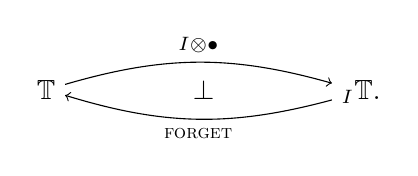
\begin{tikzpicture}[auto,baseline=(current  bounding  box.center)]
   \path[anchor=base] (0,0) node (1) {$\bT$} 
   +(4,0) node (2) {${}_I\bT.$}
   +(2,0) node (3) {$\bot$}
   ;
   \draw[->] (1) to[bend left=16] node[pos=.5,auto] {$\scriptstyle I\otimes\bullet$} (2);
   \draw[->] (2) to[bend left=16] node[pos=.5,auto] {$\scriptstyle \cat{forget}$} (1);
 \end{tikzpicture}
\end{equation}
We refer to $I$-modules in the image of the functor $I\otimes \bullet$ as {\it free}. We will see that tensoring with $I$ has the effect of ``partially semisimplifying'' $\bT$, in the following sense.

\begin{proposition}\label{pr:ss}
  For every positive integer $n$, the filtration
  \begin{equation*}
    0\subset \bC\subset Q\subset S^2Q\subset\cdots\subset S^nQ
  \end{equation*}
  splits in ${}_I\bT$ upon tensoring it with $I$. Consequently, for every $n$ the object $I\otimes S^nQ$ is injective in $\bT$. 
\end{proposition}
\begin{proof}
  We prove this inductively on $n$. For $n=1$ the claim is that the embedding
  \begin{equation*}
    I\cong I\otimes \bC\subset I\otimes Q
  \end{equation*}
  splits in ${}_I\bT$. To see this, consider the embedding
  \begin{equation*}
    Q\to \cat{forget}~I
  \end{equation*}
  in $\bT$. It corresponds, via the adjunction \Cref{eq:tit}, to a morphism in $_I\bT$
  \begin{equation*}
    {\sigma:}\ I\otimes Q\to I
  \end{equation*}
  that is clearly the identity on the $I$-submodule
  \begin{equation*}
    I\cong I\otimes \bC\subset I\otimes Q.
  \end{equation*}
  The morphism $\sigma$ is the required splitting, concluding the base case $n=1$ of the induction.

  The argument also shows that we have a decomposition
  \begin{equation}\label{eq:iqiif}
    I\otimes Q\cong I\oplus (I\otimes F) 
  \end{equation}
  in ${}_I\bT$ (and hence also in $\bT$), implying that $I\otimes Q$ is injective in $\bT$ (by \Cref{thm:hulls} for instance, which shows that both summands in \Cref{eq:iqiif} are injective).

  We regard $Q$ as a subobject of $S^2Q$ via the embedding $Q\hookrightarrow S^2Q$ described in \Cref{eq:sksk1}. By the injectivity of $I\otimes Q\in \bT$ noted above, the embedding
  \begin{equation*}
    Q\cong \bC\otimes Q\subset I\otimes Q
  \end{equation*}
  extends to a morphism in $\bT$
  \begin{equation*}
    S^2Q\to I\otimes Q. 
  \end{equation*}
  Once more, the adjunction \Cref{eq:tit} retrieves a morphism in $_I\bT$
  \begin{equation*}
    I\otimes S^2Q\to I\otimes Q
  \end{equation*}
  that restricts to the identity on the submodule
  \begin{equation}\label{formula:IQ_in_IS2Q}
    I\otimes Q\subset I\otimes S^2 Q,
  \end{equation}
  showing that the embedding \Cref{formula:IQ_in_IS2Q} splits in ${}_I\bT$. This proves the main claim for $n=2$ and the fact that there is a splitting
    \begin{equation*}
      I\otimes S^2Q\cong \left(I\otimes Q\right)\oplus \left(I\otimes S^2F\right),
    \end{equation*}
    meaning that $I\otimes S^2Q$ is injective in $\bT$. We now repeat the procedure recursively to complete the inductive argument.
\end{proof}

%In the course of the proof of \Cref{pr:ss} we have also obtained the following result, perhaps worth noting on its own for future reference.

%\begin{corollary}\label{cor.iotimessnqinjective}
 % For any non-negative integer $n$ the object $I\otimes S^nQ\in \bT$ is injective.  
 % \qedhere
%\end{corollary}

Since it will be our goal to study the category ${}_I\bT$ along the same lines as $\bT$, we next turn to simple objects therein.

\begin{theorem}\label{th:itsimp}
  The simple objects in ${}_I\bT$ are (up to isomorphism) precisely the free $I$-modules $I\otimes S$ for simples $S\in \bT$. For each of them, the endomorphism algebra in ${}_I\bT$ is $\bC$. 
\end{theorem}
\begin{proof}
  We first prove that $I\otimes S$ is simple in ${}_I\bT$. The simple objects of $\bT$ are precisely the various modules $L_{\lambda,\mu,\nu,\pi}$ of \Cref{eq:s}, and according to \Cref{thm:hulls} the injective hull $S\subset I_S$ contains $I\otimes S$ ($I_S$ exists because ${}_I \bT$ is a Grothendieck category). Since the embedding
  \begin{equation*}
    S\cong \bC\otimes S\subset I\otimes S
  \end{equation*}
  is essential in $I_S$, it is also essential in $I\otimes S$. It follows that any non-zero subobject
  \begin{equation*}
    T\subset I\otimes S
  \end{equation*}
  in ${}_I\bT$ contains $S$ and hence the $I$-module $I\otimes S$ it generates, so $T=I\otimes S$. This concludes the proof of the claim that all $I\otimes S$ are simple.

  The existence of an isomorphism
  \begin{equation}\label{eq:isomendiotimess}
    \End_{{}_I\bT}(I\otimes S)\cong \bC,
  \end{equation}
  follows from the observation that by the adjunction \Cref{eq:tit} there is an isomorphism
  \begin{equation*}
    \End_{{}_I\bT}(I\otimes S) \cong \Hom_{\bT}(S, I\otimes S). 
  \end{equation*}
  \noindent Indeed, since $I\otimes S$ is an injective hull of $S$ in $\bT$, every morphism $S\rightarrow I\otimes S$ factors through the socle $S\subset I\otimes S$, and therefore the isomorphism $\End_{\bT} S=\bC$ implies (\ref{eq:isomendiotimess}).

As for the fact that $I\otimes S$ are, up to isomorphism, all irreducible  objects in ${}_I\bT$, consider an arbitrary object $T$ and note that it must have a simple subobject $S\in \bT$. Hence $T$ must be a quotient of the (irreducible!) free object $I\otimes S\in {}_I\bT$. Consequently, we have $T\cong I\otimes S$ as desired.
\end{proof}

Since $I$ is a {\it commutative} algebra in $\bT$, the category ${}_I\bT$ of internal modules has a natural symmetric monoidal structure for which $I$ is the unit object and $\otimes_I$ is the tensor product. Whenever we refer to ${}_I\bT$ as a tensor category, this will be the structure we consider. %unless specified otherwise

%%%%%%%%%%%%%%%%%%%%%%%%%%%%%%%%%%%%%%%%%%%%%%%%%%%%%%%%%%%%%%%%%%%%%%%%%%%%%
\subsection{The category ${}_I\bT$}\label{subse:modsord}

We are now ready to apply to ${}_I\bT$ the same treatment we subjected $\bT$ to. The poset defining the Grothendieck order is obtained from the poset $(\mathcal{P},\preceq)$ of quadruples $(l,m,n,p)$ of non-negative integers with the ordering described in \Cref{eq:ord}, with the additional condition:
\begin{gather}\label{Formula new relation}
	l+m\leq l'+m' ,\quad p+n \leq p'+n' .
\end{gather}
The corresponding objects of ${_I}\mathbb{T}$ are $I_s=I\otimes J_s$ for $s\in \cP$, as in equations \Cref{eq:s} to \Cref{eq:13}.  

We will similarly consider the simple (by \Cref{th:itsimp}) objects of ${}_I\bT$
\begin{equation}\label{eq:deft}
  T_{\lambda,\mu,\nu,\pi}:=I\otimes L_{\lambda,\mu,\nu,\pi}
\end{equation}
and the semisimple objects $T_{l,m,n,p}:=I\otimes L_{l,m,n,p}$, %$s=(l,m,n,p)\in \cP$
 that are direct sums of the various $T_{\lambda,\mu,\nu,\pi}$. 

We now have the following analogue of \Cref{pr.is-ordered}.

\begin{proposition}\label{pr.itis-ordered}
${}_I\bT$ is an ordered Grothendieck category in the sense of \Cref{def.ord-gr}.   
\end{proposition}
\begin{proof}
  Taking as above the objects $X_s$ to be our $I_s$ (this time regarded as objects in ${}_I\bT$ rather than just $\bT$), the argument proceeds much as in the proof of \Cref{pr.is-ordered} with a small difference in how we define the morphisms $I_s\to I_t$ for $t\prec s$ from \Cref{def.ord-gr}, (\labelcref{item:9}).

  Once again, said morphisms will be tensor products and compositions of a few building blocks:
  \begin{itemize}
  \item[$-$] projecting one of the tensorands $V^*$ of $I_s=J_s\otimes I$ onto $W_*$;
  \item[$-$] the dual analogue, $V^*_*\to W$;
  \item[$-$] the ``pairing''
    \begin{equation}\label{eq:realpair}
      I_{0,1,0,0}\otimes_I I_{0,0,1,0} = (I\otimes V^*)\otimes_{I} (I\otimes V_*^*)\cong I\otimes V^*\otimes V_*^*\to I
    \end{equation}
    obtained via the adjunction \Cref{eq:tit} from the composition
    \begin{equation*}
      V^*\otimes V_*^*\to Q\subset I
    \end{equation*}
    in \Cref{eq:partpair}. 
  \end{itemize}
  Everything else goes through as sketched in the proof of \Cref{pr.is-ordered}. 
\end{proof}


The difference from $\bT$ is that now the free $I$-modules generated by the full duals $V^*$ and $V_*^*$ admit the pairing \Cref{eq:realpair} valued in the {\it unit object} $I$ of the category ${}_I\bT$ under consideration. 


We also have an $I$-module version of \Cref{thm:hulls}. 

\begin{theorem}\label{thm:ihulls}
    For every quadruple $(\lambda,\mu,\nu,\pi)$ of Young diagrams, the inclusion
  \begin{equation*}
    T_{\lambda,\mu,\nu,\pi} = I\otimes L_{\lambda,\mu,\nu,\pi} \subseteq I_{\lambda,\mu,\nu,\pi} = I\otimes J_{\lambda,\mu,\nu,\pi}
  \end{equation*}
  obtained by applying the functor $I\otimes \bullet$ to the inclusion
  \begin{equation*}
    L_{\lambda,\mu,\nu,\pi} \subseteq J_{\lambda,\mu,\nu,\pi}
  \end{equation*}
  is an injective hull in ${}_I\bT$.
  \qedhere
\end{theorem}


Just as $\bT$, the category ${}_I\bT$ can be realized as comodules over a coalgebra (see \Cref{th:koszcoalg}). As in that previous result, we denote by ${}_I\bT_{fin}\subset {}_I\bT$ the full subcategory of finite-length objects. Note that the indecomposable injectives
\begin{equation*}
I_{\lambda,\mu,\nu,\pi} = I\otimes J_{\lambda,\mu,\nu,\pi}  \in {}_I\bT
\end{equation*}
have finite length: $J_{\lambda,\mu,\nu,\pi}$ have finite filtrations with subquotients simple in $\bT$, and according to \Cref{th:itsimp} tensoring these simple objects by $I$ produces simples in ${}_I\bT$.

\begin{theorem}\label{th:ikoszcoalg}
  The Grothendieck category ${}_I{\bT}$ is equivalent to the category $\cM^D$ of comodules over a coalgebra $D$, with ${}_I\bT_{fin}\simeq \cM^D_{fin}$. Furthermore, the coalgebra $D$ is left semiperfect in the sense of \Cref{def:perf}. 
\end{theorem}
\begin{proof}
  The argument is largely parallel to that underpinning \Cref{th:koszcoalg}, via \Cref{thm:tak} (minus Koszulity, which we have not yet addressed for $I$-modules).

  The additional remark, that $D$ is semiperfect, follows directly from \Cref{def:perf} and the fact that, as observed above, in ${}_I\bT$ the indecomposable injectives $I_{\lambda,\mu,\nu,\pi}$ have finite length.
\end{proof}


We also need the following remark, which parallels \cite[Lemma 2.19]{us0} (the proof is virtually identical, so we omit it).

\begin{lemma}\label{le:fullonx}
  The tensor subcategory ${}_I\bT'$ of ${}_I\bT$ generated by the morphisms described in the proof of \Cref{pr.itis-ordered} is the full subcategory containing $I_{l,m,n,p}$.  \qedhere
\end{lemma}

We next turn to the Koszulity of ${}_I\bT$. In keeping with the theme, the argument will be very similar to what we saw in proving \Cref{thm:right-def,thm:4kosz}. %We collect all of the statements together as follows.

\begin{theorem}\label{th:ikosz}
  The Grothendieck category ${}_I\bT$ is sharp in the sense of \Cref{def.shrp}: for any two simples $S,T\in {\bT}$ we have
  \begin{equation*}
    \mathrm{Ext}^q(S,T)\ne 0\quad \Rightarrow\quad  d(s,t)=q.
  \end{equation*}
  In particular, the ordered Grothendieck category ${}_I\bT$ is Koszul in the sense of \Cref{def.ksz}.
\end{theorem}
\begin{proof}
The last claim follows from sharpness by \Cref{thm:kosz-gen}, so we focus on proving the sharpness claim. In turn, the latter follows as in the proof of \Cref{thm:right-def}, with the exact sequence \Cref{eq:18} replaced by its analogue, obtained by simply tensoring it with $I$.   
\end{proof}


\begin{remark}
  Note that in the present setting the proof of Koszulity is in fact simpler than in \Cref{subse:kosz}: we do not need a version of \Cref{pr.thk}, since for purely thick simple objects $L_{\lambda,\emptyset,\emptyset,\pi}$ the corresponding simple object of ${}_{I}\bT$
  \begin{equation*}
    T_{\lambda,\emptyset,\emptyset,\pi} = I\otimes L_{\lambda,\emptyset,\emptyset,\pi}
  \end{equation*}
  is injective. 
\end{remark}

As a consequence, we can supplement \Cref{th:ikoszcoalg}, fully bringing it in line with \Cref{th:koszcoalg}. 

\begin{corollary}\label{cor.dgradedkoszul}
The coalgebra $D$ in \Cref{th:ikoszcoalg} can be chosen graded and Koszul. 
  \qedhere
\end{corollary}

We end the present subsection with description of one possible choice for the graded coalgebra $C$ from \Cref{th:koszcoalg}. This discussion parallels \cite[\S 3.4]{us0}, which in turn is analogous to \cite[\S 5]{DPS}.



Let $T$ be the tensor algebra in ${}_I\bT$ of the object
\begin{equation*}
  (W_*\otimes I)\oplus (V^*\otimes I)\oplus (V_*^*\otimes I)\oplus (W\otimes I)  = I_{1,0,0,0}\oplus I_{0,1,0,0}\oplus I_{0,0,1,0}\oplus I_{0,0,0,1}
\end{equation*}
with $T_d$ denoting its degree-$d$ component, and the non-unital algebra of endomorphisms
\begin{equation*}
  \mathcal{A}:=\bigoplus_{m,n\in \bZ_{\ge 0}}\Hom_{{}_I\bT}(T_m,T_n)\label{eq:a}=\bigoplus_{s,t\in \cP}\Hom_{{}_I\bT}(I_s, I_t).
\end{equation*}
The algebra $\mathcal{A}$ is naturally $\bZ_{\ge 0}$-graded by means of the defect introduced in \Cref{def:defect}:
\begin{equation*}
  \mathcal{A}_d:=\bigoplus_{\substack{s,t\in \cP \\ d(t,s)=d}}\Hom_{{}_I\bT}(I_s, I_t).
\end{equation*}
Finally, the coalgebra $C$ is simply the graded dual of $\mathcal{A}$, with $C_d=\mathcal{A}_d^*$.

The fact that $C$ (and hence $\mathcal{A}$) is Koszul then implies

\begin{proposition}\label{pr:isquad}
  The algebra $\mathcal{A}$ is quadratic. 
\end{proposition}
\begin{proof}
  Koszul algebras are well known to be quadratic; see e.g. \cite[\S 2.3]{BGS}.
\end{proof}

%%%%%%%%%%%%%%%%%%%%%%%%%%%%%%%%%%%%%%%%%%%%%%%%%%%%%%%%%%%%%%%%%%%%%%%%%%%%%
\subsection{Universality}\label{subse:univ}

We can now characterize ${}_I\bT$ as a universal category in the sense of \cite[Theorem 4.23]{us0} and \cite[Theorem 5.2]{us1}. First, note that in ${}_I\bT$ there is a pairing
\begin{equation}\label{eq:pairi}
  (I\otimes V^*)\otimes_I (I\otimes V_*^*)\cong I\otimes V^*\otimes V_*^*\to I
\end{equation}
corresponding to \Cref{eq:partpair} through the adjunction \Cref{eq:tit}. We will occasionally indicate tensoring with $I$ by a left-hand `$I$' subscript, as in ${}_IX:= I\otimes X$.

\begin{theorem}\label{th:sl-univ}
  Let $(\cD,\ \otimes,\ {\bf 1})$ be a ($\bC$-linear abelian) tensor category, $x\hookrightarrow x_*^*$ and $x_*\hookrightarrow x^*$ be monomorphisms in $\cD$, and
  \begin{equation*}
    p: x^*\otimes x_*^*\to {\bf 1}
  \end{equation*}
  be a morphism in $\cD$.

  \begin{enumerate}[(a)]
  \item There is a unique (up to monoidal natural isomorphism) left exact symmetric monoidal functor $F:{}_I\bT_{fin}\to \cD$ sending
    \begin{itemize}
    \item[$-$] the pairing \Cref{eq:pairi} to $p$;
    \item[$-$] the surjection ${}_IV_*^*\to {}_IW$ to $x_*^*\to x_*^*/x$;
    \item[$-$] the surjection ${}_IV^*\to {}_IW_*$ to $x^*\to x^*/x_*$. 
    \end{itemize}
  \item if $\cD$ is additionally a Grothendieck category then $F$ extends uniquely to a coproduct-preserving functor ${}_I\bT\to \cD$.
  \end{enumerate}
\end{theorem}

The argument will be analogous to that employed in the proof of \cite[Theorem 3.23]{us0}, revolving around the fact that the algebra $A$ in the preceding discussion is quadratic (\Cref{pr:isquad}). For that reason, it will be necessary to understand its components of degree $\le 2$. In degree zero things are simple: the following result is the version of \cite[Lemma 3.24]{us0} appropriate here.

\begin{lemma}\label{le:deg0}
  For $(l,m,n,p)\in \cP$ the endomorphism algebra of the injective object $I_{l,m,n,p}\in {}_I\bT$ is isomorphic to $\bC[S_l\times S_m\times S_n\times S_p]$, with the symmetric groups acting naturally on the relevant tensorands of
  \begin{align*}
    I_{l,m,n,p} &= I\otimes J_{l,m,n,p}\\
                &=I\otimes W_*^{\otimes l}\otimes (V^*)^{\otimes m}\otimes (V_*^*)^{\otimes n} \otimes W^{\otimes p}.
  \end{align*}
\end{lemma}
\begin{proof}
  We have
  \begin{equation*}
    \End_{{}_I\bT}(I\otimes J_{l,m,n,p})\cong \Hom_{\bT}(J_{l,m,n,p},I\otimes J_{l,m,n,p}). 
  \end{equation*}
  The quotient of $J_{l,m,n,p}$ by its socle in $\bT$ has a filtration by subquotients $L_{\lambda',\mu',\nu',\pi'}$ with
  \begin{equation*}
    (|\lambda'|,|\mu'|,|\nu'|,|\pi'|) \prec (l,m,n,p)\in \cP,
  \end{equation*}
  which thus admit no non-zero morphisms to
  \begin{equation*}
    \mathrm{soc}(I\otimes J_{l,m,n,p} )= \mathrm{soc}J_{l,m,n,p}. 
  \end{equation*}
  It follows that restricting an arbitrary morphism 
  \begin{equation*}
    J_{l,m,n,p}\to I\otimes J_{l,m,n,p}
  \end{equation*}
  in $\bT$ to the socle induces an isomorphism
  \begin{equation}\label{eq:homend}
    \Hom_{\bT}(J_{l,m,n,p},I\otimes J_{l,m,n,p})
    \cong
    \End_{\bT}\left(W_*^{\otimes l}\otimes (V^*)^{\otimes m}\otimes (V_*^*)^{\otimes n} \otimes W^{\otimes p}\right). 
  \end{equation}
  We can see that the right-hand side of \Cref{eq:homend} is naturally identifiable with $\bC[S_l\times S_m\times S_n\times S_p]$ as in \Cref{pr:gpendoalgs}.
\end{proof}

As for degree $1$, we need an analogue of \cite[Lemma 3.25]{us0}. Stating such an analogue will require some notation. Degree-one morphisms between the objects $I_{l,m,n,p}\in {}_I\bT$ come in three flavors:
\begin{align*}
  I_{l,m,n,p}&\to I_{l,m-1,n-1,p},\\
  I_{l,m,n,p}&\to I_{l+1,m-1,n,p},\\
  I_{l,m,n,p}&\to I_{l,m,n-1,p+1}.
\end{align*}
We distinguish families of each flavor, as follows. The morphism
\begin{equation*}
  \phi_{i,j}:I_{l,m,n,p}\to I_{l,m-1,n-1,p}\ \text{ for } 1\le i \le m,~1\le j \le n
\end{equation*}
executes the pairing
\begin{equation*}
  V^*\otimes V_*^*\to I
\end{equation*}
of the $i^{th}$ tensorand $V^*$ and the $j^{th}$ tensorand $V_*^*$ in
\begin{equation*}
  I_{l,m,n,p} = I\otimes W_*^{\otimes l}\otimes (V^*)^{\otimes m}\otimes (V_*^*)^{\otimes n} \otimes W^{\otimes p}
\end{equation*}
and acts as the identity on all other tensorands.

Next, we have the map
\begin{equation*}
{}_{i,j}\pi:I_{l,m,n,p}\to I_{l+1,m-1,n,p}\ \text{ for } 1\le i \le m,~1\le j \le n
\end{equation*}
which
\begin{itemize}
\item[$-$] first permutes cyclically the first $i$ tensorands $V^*$;
\item[$-$] maps the new first (old $i^{th}$) tensorand $V^*$ onto $W_*=V^*/V_*$;
\item[$-$] finally permutes the last $m-j+1$ tensorands $W^*$ cyclically so the newly-created $W_*$ becomes the $j^{th}$.
\end{itemize}

Finally, we have the left-right mirror image 
\begin{equation*}
\pi_{i,j}:I_{l,m,n,p}\to I_{l,m,n-1,p+1}\ \text{ for } 1\le i \le m,~1\le j \le n
\end{equation*}
of ${}_{i,j}\pi$, obtained by substituting $V_*^*$ for $V^*$, $W$ for $W_*$, reversing the directions of the cyclic permutations, etc.


We write
\begin{equation*}
  S_{l,m,n,p}:=S_l\times S_m\times S_n\times S_p
\end{equation*}
for products of symmetric groups and, unless specified otherwise, morphism spaces in \Cref{le:deg1} below are in the category ${}_I\bT$. 

\begin{lemma}\label{le:deg1}
  Let $(l,m,n,p)\in \cP$.
  \begin{enumerate}[(a)]
  \item\label{item:16} $\Hom(I_{l,m,n,p},I_{l,m-1,n-1,p})$ is isomorphic to $\bC[S_{l,m,n,p}]$ as a bimodule over
    \begin{equation*}
      \End I_{l,m-1,n-1,p} \cong \bC [S_{l,m-1,n-1,p} ]\text{ and }\End I_{l,m,n,p}\cong \bC [S_{l,m,n,p}],
    \end{equation*}
    with any of the morphisms $\phi_{i,j}$ as a generator for the right $\bC [S_{l,m,n,p} ]$-module structure while identifing the subgroups
    \begin{equation*}
     S_{m-1}\subset S_{m} \text{ and } S_{n-1} \subset S_{n}
    \end{equation*}
     with the isotropy groups of $i$ and $j$ respectively. 
  \item\label{item:17} $\Hom(I_{l,m,n,p},I_{l+1,m-1,n,p})$ is isomorphic to the induced module
    \begin{equation*}
      \bC [S_{l+1,m,n,p}]\cong \mathrm{Ind}_{S_l}^{S_{l+1}} \bC [S_{l,m,n,p}] = \bC [S_{l+1}]\otimes_{\bC [S_l]}\bC [S_{l,m,n,p}]
    \end{equation*}
    as a bimodule over
    \begin{equation*}
      \End I_{l+1,m-1,n,p}\cong \bC [S_{l+1,m-1,n,p}]\text{ and }\End I_{l,m,n,p} \cong \bC [S_{l,m,n,p}],
    \end{equation*}
    with ${}_{i,j}\pi$ as a generator for the right $\bC [S_{l,m,n,p}]$-module structure while identifying the subgroups
    \begin{equation*}
      S_l\subset S_{l+1}\text{ and } S_{m-1}\subset S_m
    \end{equation*}
    with the isotropy groups of $j$ and $i$ respectively. 
  \item\label{item:18} The left-right mirror image of \Cref{item:17}: $\Hom(I_{l,m,n,p},I_{l,m,n-1,p+1})$ is isomorphic to the induced module
    \begin{equation*}
      \bC [S_{l,m,n,p+1}]\cong \mathrm{Ind}_{S_p}^{S_{p+1}} \bC [S_{l,m,n,p}] = \bC [S_{p+1}]\otimes_{\bC [S_p]}\bC [S_{l,m,n,p}]
    \end{equation*}
    as a bimodule over
    \begin{equation*}
      \End I_{l,m,n-1,p+1}\cong \bC [S_{l,m,n-1,p+1}]\text{ and }\End I_{l,m,n,p}\cong \bC [S_{l,m,n,p}],
    \end{equation*}
    with $\pi_{i,j}$ as a generator for the right $\bC [S_{l,m,n,p}]$-module structure while identifying the subgroups
    \begin{equation*}
      S_p\subset S_{p+1}\text{ and } S_{n-1}\subset S_n
    \end{equation*}
    with the isotropy groups of $j$ and $i$ respectively. 
  \end{enumerate}
\end{lemma}
\begin{proof}  
  {\Cref{item:16}} Having fixed $i$ and $j$ as in the statement, we have a morphism
  \begin{equation}\label{eq:mnm1n1}
    \bC [S_{l,m,n,p}]\to \Hom(I_{l,m,n,p},I_{l,m-1,n-1,p})
  \end{equation}
  of $(\bC[S_{l,m-1,n-1,p}], \bC[S_{l,m,n,p}])$-bimodules, sending $1$ to $\phi_{i,j}$. \Cref{le:fullonx} implies that this morphism is surjective, so it is the injectivity that we focus on.   

  Note that the morphism \Cref{eq:mnm1n1} factors as
  \begin{equation}\label{eq:largediag}
    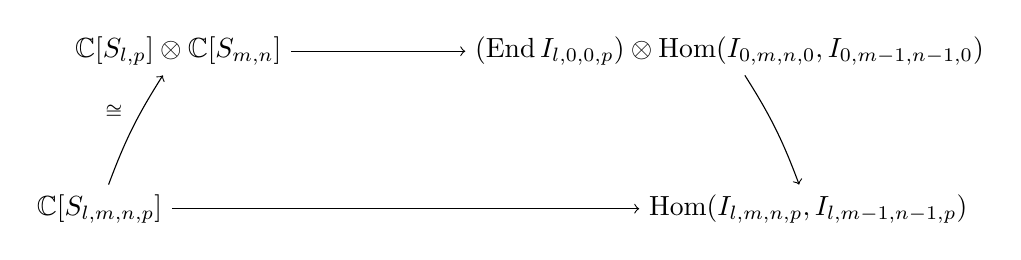
\begin{tikzpicture}[auto,baseline=(current  bounding  box.center)]
      \path[anchor=base] 
      (0,0) node (l) {$\bC [S_{l,m,n,p}]$}
      +(1,2) node (ul) {$\bC [S_{l,p}]\otimes \bC [S_{m,n}]$}
      +(8,2) node (ur) {$(\End I_{l,0,0,p})\otimes \Hom(I_{0,m,n,0},I_{0,m-1,n-1,0})$}
      +(9,0) node (r) {$\Hom(I_{l,m,n,p},I_{l,m-1,n-1,p})$}
      ;
      \draw[->] (l) to[bend left=6] node[pos=.5,auto] {$\scriptstyle \cong$} (ul);
      \draw[->] (ul) to[bend left=0] node[pos=.5,auto] {$\scriptstyle $} (ur);
      \draw[->] (ur) to[bend left=6] node[pos=.5,auto,swap] {$\scriptstyle $} (r);
      \draw[->] (l) to[bend right=0] node[pos=.5,auto,swap] {$\scriptstyle $} (r);
    \end{tikzpicture}
  \end{equation}
  where the downward arrow is the tensor product (over the unit object $I\in {}_I\bT$) of morphisms in ${}_I\bT$. Since the vertical maps are injective, the bottom morphism (which is in our focus) will be one-to-one if and only if the top arrow is. The left-hand tensorand
  \begin{equation*}
    \bC [S_{l,p}]\to \End I_{l,0,0,p}
  \end{equation*}
  of the top map in \Cref{eq:largediag} is an isomorphism by \Cref{le:deg0}, so it is enough to consider the right hand tensorand
  \begin{equation*}
    \bC [S_{m,n}]\to \Hom(I_{0,m,n,0},I_{0,m-1,n-1,0})
  \end{equation*}
  of that map; equivalently, it suffices to resolve the present discussion in the case $l=p=0$. But this follows from \cite[Lemma 3.25 (a)]{us0} (which is analogous to the result being proven here), by noting that the restrictions of the compositions
  \begin{equation*}
    \phi_{i,j}\circ \sigma: I_{0,m,n,0}\to I_{0,m-1,n-1,0},\quad \sigma\in S_{m,n}
  \end{equation*}
  to
  \begin{equation*}
    (V^*)^{\otimes m}\otimes V^{\otimes n}\subset (V^*)^{\otimes m}\otimes (V_*^*)^{\otimes n}\subset I_{0,m,n,0}
  \end{equation*}
  are precisely the morphisms proven linearly independent there. 

  {\Cref{item:17}} We again have an $(\bC[S_{l+1,m-1,n,p}],\bC[S_{l,m,n,p}])$-bimodule map
  \begin{equation}\label{eq:lml1m1}
    \bC [S_{l+1,m,n,p}] \to \Hom(I_{l,m,n,p},I_{l+1,m-1,n,p})
  \end{equation}
  sending $1$ to ${}_{i,j}\pi$, and its surjectivity is a consequence of \Cref{le:fullonx}. The injectivity follows as in part \Cref{item:16}, by first decomposing \Cref{eq:lml1m1} as a tensor product of maps
  \begin{equation*}
    \bC [S_{l+1,m}] \to \Hom(I_{l,m,0,0},I_{l+1,m-1,0,0})
  \end{equation*}
  and
  \begin{equation*}
    \bC [S_{n,p}] \to \End I_{0,0,n,p}. 
  \end{equation*}
  The latter is an isomorphism by \Cref{le:deg0}, and the former is an injection as in the proof of \Cref{item:16}, by appealing to \cite[Lemma 3.25 (b)]{us0}. 
  
  {\Cref{item:18}} As noted in the statement, this is entirely parallel to part \Cref{item:17}, interchanging the roles of $V^*$ and $V_*^*$, $l$ and $p$, $m$ and $n$, etc.
\end{proof}

% % As for the quadratic relations satisfied by the degree-$1$ elements described by \Cref{le:deg1}, we begin with the following result, parallel to \cite[Lemma 3.26]{us0}, describing the two-fold tensor products of the degree-$1$ spaces in \Cref{le:deg1} over the degree-$0$ spaces in \Cref{le:deg0}. Once more, all unadorned morphism spaces are in the category ${}_I\bT$.
% %

The composition map from the degree-one to the degree-two component of $A$ comes in several varieties, depending on the domain. Before listing the various options, it will be convenient to introduce

\begin{notation}\label{not:iud}
  For a quadruple $(l,m,n,p)\in \cP$ we write
  \begin{equation*}
    I_{l,m\downarrow,n\downarrow,p}:=\Hom_{{}_I\bT}(I_{l,m,n,p},I_{l,m-1,n-1,p})
  \end{equation*}
  and similarly for other morphism spaces, with arrows indicating whether the respective index increases or decreases, and multiple arrows to indicate the amount. Other examples are
  \begin{align*}
    I_{l,m\downarrow\downarrow,n\downarrow\downarrow,p}&:=\Hom_{{}_I\bT}(I_{l,m,n,p},I_{l,m-2,n-2,p}){,}\\
    I_{l\uparrow,m\downarrow,n,p}&:=\Hom_{{}_I\bT}(I_{l,m,n,p},I_{l+1,m-1,n-2,p})\\
  \end{align*}
  and so on.

  For composable morphism spaces in ${}_I\bT$ we denote by `$\odot$' the tensor product over the endomorphism algebra of the intermediate object. For example:
  \begin{equation*}
    I_{l,(m-1)\downarrow,(n-1)\downarrow,p}\odot I_{l,m\downarrow,n\downarrow,p}
    :=
    I_{l,(m-1)\downarrow,(n-1)\downarrow,p}\otimes_{\bC [S_{l,m-1,n-1,p}]} I_{l,m\downarrow,n\downarrow,p}{.}
  \end{equation*}
\end{notation}


% % recall \Cref{not:mor}; here, the category $\cC$ in that notational convention is taken to be ${}_I\bT$ unless specified otherwise.
% % 

With this in place, the possibilities for composition of degree-1 morphisms are:

\begin{equation}\label{eq:22}
  I_{l,(m-1)\downarrow,(n-1)\downarrow,p}\odot I_{l,m\downarrow,n\downarrow,p}
  \to
  I_{l,m\downarrow\downarrow,n\downarrow\downarrow,p},
\end{equation}

which is mirror-self-dual,

\begin{equation}\label{eq:23}
  I_{(l+1)\uparrow,(m-1)\downarrow,n,p}\odot I_{l\uparrow,m\downarrow,n,p}
  \to
  I_{l\uparrow\uparrow,m\downarrow\downarrow,n,p}
\end{equation}

and its mirror image

\begin{equation}\label{eq:24}
  I_{l,m,(n-1)\downarrow,(p+1)\uparrow}\odot I_{l,m,n\downarrow,p\uparrow}
  \to
  I_{l,m,n\downarrow\downarrow,p\uparrow\uparrow},
\end{equation}


\begin{equation}\label{eq:25}
  (I_{l\uparrow,(m-1)\downarrow,n-1,p}\odot I_{l,m\downarrow,n\downarrow,p})
  \oplus
  (I_{l+1,(m-1)\downarrow,n\downarrow,p}\odot I_{l\uparrow,m\downarrow,n,p})
  \to
  I_{l\uparrow,m\downarrow\downarrow,n\downarrow,p}
\end{equation}

and its mirror image 

\begin{equation}\label{eq:26}
  (I_{l,m-1,(n-1)\downarrow,p\uparrow}\odot I_{l,m\downarrow,n\downarrow,p})
  \oplus
  (I_{l,m\downarrow,(n-1)\downarrow,p+1}\odot I_{l,m,n\downarrow,p\uparrow})
  \to
  I_{l,m\downarrow,n\downarrow\downarrow,p\uparrow},
\end{equation}

and finally, the self-dual morphism

\begin{equation}\label{eq:27}
  (I_{l+1,m-1,n\downarrow,p\uparrow}\odot I_{l\uparrow,m\downarrow,n,p}
)  \oplus
  (I_{l\uparrow,m\downarrow,n-1,p+1}\odot I_{l,m,n\downarrow,p\uparrow})
  \to
  I_{l\uparrow,m\downarrow,n\downarrow,p\uparrow}.
\end{equation}


The nine `$\odot$' symbols above account for the nine possible ways of composing two morphisms, each being of one of the three flavors listed in \Cref{le:deg1}. 

\begin{remark}
  Note that in all cases the product `$\odot$' conserves the total number of up as well as down arrows.
\end{remark}


% % \begin{lemma}\label{le:deg2base}
% % 
% % \end{lemma}
% % \begin{proof}
% %   This is an immediate consequence of \Cref{le:deg1}.
% % \end{proof}
% % 
% % 
% % \begin{lemma}\label{le:deg2rels}
% %   
% % \end{lemma}
% % \begin{proof}
% % 
% % 
% %   \alex{do}
% % \end{proof}
% % 

\pf{th:sl-univ}
\begin{th:sl-univ}[sketch]
  As in the proof of \cite[Theorem 3.23]{us0}, an appeal to \cite[Theorem 2.22]{us0} together with \Cref{pr.itis-ordered} proves the statement as soon as we argue that the initial data of
  \begin{align*}
    x\hookrightarrow x_*^*, ~x_*\hookrightarrow x^*\text{ and}~p:x^*\otimes x_*^*\to {\bf 1}
  \end{align*}
  in the tensor category $\cD$ extends to a linear monoidal functor
  \begin{equation*}
    F:{}_I\bT'\to \cD,
  \end{equation*}
  where ${}_I\bT'$ is, as in \Cref{le:fullonx}, the full subcategory of ${}_I\bT$ on the objects $I_{l,m,n,p}$. Set ${}_I T:=T\otimes I$ for any $T\in \bT$. Since the objects of ${}_I\bT'$ are precisely the tensor powers (over $I\in {}_I\bT$) and the morphisms are tensor products and compositions of permutation of tensorands, evaluations \Cref{eq:pairi}, inclusions ${}_IV_*\subset {}_IV^*$ and ${}_IV\subset {}_IV_*^*$, etc., there is an obvious candidate for such an extension $F$, sending
  \begin{align*}
    {}_IV_*^*&\mapsto x_*^*\quad\text{and}\quad {}_IW\mapsto x_*^*/x,\\
    {}_IV^*&\mapsto x^*\quad\text{and}\quad {}_IW_*\mapsto x^*/x_*,\\
    \text{\Cref{eq:pairi}}&\mapsto p,
  \end{align*}
  etc. What we have to argue is that that extension is in fact well defined.

  The fact that, by \Cref{pr:isquad}, the algebra $\mathcal{A}$ defined in Section \ref{eq:a} is quadratic, means that it will be enough to check that the degree-two relations between degree-one morphisms between the $I_{l,m,n,p}$ (i.e. the kernels of the maps \Cref{eq:22,eq:23,eq:24,eq:25,eq:26,eq:27}) vanish in $\cD$ upon substituting $x$ for ${}_IV$, $x_*$ for ${}_IV_*$, etc. This would be a somewhat tedious and unenlightening check if done exhaustively, so we exemplify the argument by treating \Cref{eq:22} alone. In that regard, we make the claim:

 {\it The kernel of the composition \Cref{eq:22} is generated, as an $(S_{l,m-2,n-2,p},S_{l,m,n,p})$-bimodule, by
    \begin{equation}\label{eq:inker}
      \phi_{m-1,n-1}\otimes \phi_{m,n} - \phi_{m-1,n-1}\otimes \phi_{m,n}\circ (m,m-1)(n,n-1),
    \end{equation}
    where $(m,m-1)$ is the respective transposition in $S_m\subset S_{l,m,n,p}$ and similarly,
    \begin{equation*}
      (n,n-1)\in S_n\subset S_{l,m,n,p}. 
    \end{equation*}
  }
  
  Assuming the claim for now, we observe that the relations annihilated by \Cref{eq:22} hold in any tensor category. It follows that our candidate functor $F$ is indeed compatible with the quadratic relations imposed by composition, and hence is well defined. It thus remains to prove the claim; this is the goal we focus on for the duration of the present proof, following the layout of the proof of \cite[Lemma 3.27 (a)]{us0}.

  First, note that the morphism \Cref{eq:22} is surjective by \Cref{le:fullonx}. Secondly, the fact that \Cref{eq:inker} belongs to the kernel of \Cref{eq:22} is immediate: this is because %that formula simply says that
  \begin{itemize}
  \item[$-$] evaluating the $m^{th}$ tensorand ${}_IV^*$ against the $n^{th}$ tensorand ${}_IV_*^*$, and then
  \item[$-$] evaluating the $(m-1)^{st}$  tensorand ${}_IV^*$ against the $(n-1)^{st}$  tensorand ${}_IV_*^*$
  \end{itemize}

  has the same effect as

  \begin{itemize}
  \item[$-$] permuting the $m^{th}$ and $(m-1)^{st}$ tensorands ${}_IV^*$,
  \item[$-$] permuting the $n^{th}$ and $(n-1)^{st}$ tensorands ${}_IV_*^*$
  \end{itemize}
  and then repeating the two evaluations above.

  The proof will thus be complete if we argue that the kernel of \Cref{eq:22} is not {\it strictly} larger than the bimodule generated by \Cref{eq:inker}. We do this by a dimension count. Tensoring two instances of \Cref{le:deg1}, \Cref{item:16} over $\bC [S_{l,m-1,n-1,p}]$, we conclude that the domain
  \begin{equation*}
    I_{l,(m-1)\downarrow,(n-1)\downarrow,p}\odot I_{l,m\downarrow,n\downarrow,p}
  \end{equation*}
  of \Cref{eq:22} is isomorphic to $\bC [S_{l,m,n,p}]$ as an $(\bC[S_{l,m-2,n-2,p}],\bC[S_{l,m,n,p}])$-bimodule, with
  \begin{itemize}
  \item[$-$] $\phi_{m,n}$ identified with the generator $1\in \bC [S_{l,m,n,p}]$, and
  \item[$-$] $S_{l,m-2,n-2,p}\subset S_{l,m,n,p}$ being the subgroup fixing $m$, $m-1$, $n$ and $n-1$. 
  \end{itemize}

  This identification turns the putative generator \Cref{eq:inker} of the kernel of \Cref{eq:22} into
  \begin{equation}\label{eq:elem}
    1-(m,m-1)(n,n-1)\in \bC [S_{l,m,n,p}].
  \end{equation}
  The $(\bC[S_{l,m-2,n-2,p}],\bC[S_{l,m,n,p}])$-bimodule generated by \Cref{eq:elem} coincides with the right $S_{l,m,n,p}$-module generated by the same element. The dimension of that module is half that of $\bC [S_{l,m,n,p}]$, and hence
  \begin{equation*}
    \dim \ker ~\text{\Cref{eq:22}} = \frac 12 l!m!n!p! = \frac 12 \left(\dim~\text{domain of \Cref{eq:22}}\right).
  \end{equation*}
  The desired conclusion that the kernel of the surjection \Cref{eq:22} cannot strictly contain the bimodule generated by \Cref{eq:inker} will thus follow if we prove that
  \begin{equation*}
    \dim I_{l,m\downarrow\downarrow,n\downarrow\downarrow,p} = \dim \Hom(I_{l,m,n,p},I_{l,m-2,n-2,p})\ge \frac 12 l!m!n!p!{.}
  \end{equation*}

  Since we have an embedding
  \begin{equation*}
    (\End I_{l,0,0,p})\otimes I_{0,m\downarrow\downarrow,n\downarrow\downarrow,0}\to I_{l,m\downarrow\downarrow,n\downarrow\downarrow,p}
  \end{equation*}
  and the left-hand tensorand is isomorphic to $\bC [S_{l,p}]$ by \Cref{le:deg0}, it is enough to assume that $l=p=0$ and show that
  \begin{equation*}
    \dim \Hom_{{}_I\bT}\left(({}_IV^*)^{\otimes m}\otimes_I ({}_IV_*^*)^{\otimes n}, ({}_IV^*)^{\otimes (m-2)}\otimes_I ({}_IV_*^*)^{\otimes (n-2)}\right)
    \ge
    \frac 12 m! n!,
  \end{equation*}
  or equivalently, via the adjunction \Cref{eq:tit}, that 
    \begin{equation*}
    \dim \Hom_{\bT}\left((V^*)^{\otimes m}\otimes (V_*^*)^{\otimes n}, I\otimes (V^*)^{\otimes (m-2)}\otimes (V_*^*)^{\otimes (n-2)}\right)
    \ge
    \frac 12 m! n!.
  \end{equation*}  
  This, however, follows by restricting the morphisms on the left to $V_*^{\otimes m}\otimes V^{\otimes n}$ and noting that we already know the analogous inequality
  \begin{equation*}
    \dim \Hom_{\bT}\left(V_*^{\otimes m}\otimes V^{\otimes n}, V_*^{\otimes (m-2)}\otimes V^{\otimes (n-2)}\right)
    \ge
    \frac 12 m! n!
  \end{equation*}
  from the computation carried out in \cite[Lemma 6.3]{DPS}, or from \cite[Lemma 3.27 (a)]{us0} (which is analogous to the claim being proven here).
\end{th:sl-univ}

%%%%%%%%%%%%%%%%%%%%%%%%%%%%%%%%%%%%%%%%%%%%%%%%%%%%%%%%%%%%%%%%%%%%%%%%%%%%%
%%%%%%%%%%%%%%%%%%%%%%%%%%%%%%%%%%%%%%%%%%%%%%%%%%%%%%%%%%%%%%%%%%%%%%%%%%%%%
\section{Orthogonal and symplectic analogues of the categories $\bT$ and ${}_I\bT$}\label{se:bcd}

In this final section we discuss briefly the orthogonal and symplectic versions of the categories $\bT$ and $_I \bT$. The orthogonal and symplectic analogues of the Lie algebra $\fgl^M(V,V_*)$ are the Lie algebras $\fo(V)$ and $\fs\fp(V)$ where $V$ is now equipped with a nondegenerate symmetric or antisymmetric bilinear form $\langle \cdot, \cdot \rangle:V\times V \rightarrow \mathbb{C}$, yielding a respective linear map $S^2 V\rightarrow \bC$ or $\Lambda^2 V \rightarrow \bC$. The Lie algebras $\fo(V)$ and $\fs\fp(V)$ are defined as the respective largest subalgebras of $\fgl^M(V,V)$ for which the map $S^2 V\rightarrow \bC$ or $\Lambda^2 V \rightarrow \bC$ is a morphism of representations.

Let $\fg=\fo(V)$, $\fs\fp(V)$. Then $V$ is a submodule of $V^*$ (via the form $\langle \cdot,\cdot\rangle$), and the $\fg$-module $W:=V^*/V$ is irreducible. This can be proved for instance by considering $W$ over the family of Lie subalgebras $\fgl^M(V',V'_*)\subset \fg$ arising from varying decompositions of $V$ as $V'\oplus V'_{*}$ for maximal isotropic subspaces $V'$, $V'_{*}$. Over each such subalgebra $W$ is isomorphic to \begin{equation*}
V'^*/V_*\oplus (V_*)^*/V,
\end{equation*} and hence has precisely two proper submodules. Since these submodules vary when $V'$ and $V'_*$ vary, the module $W$ is irreducible over $\fg$.

 Furthermore, for any Young diagram $\lambda$, the irreducible $\fgl^M(V,V)$-module $V_{\lambda}$ restricts to $\fg$ yielding a generally reducible $\fg$-module. In all cases the socle of $V_{\lambda}|_{\fg}$ is simple, and we denote it by $V_{[\lambda]}$ for $\fg=\fo(V)$ and by $V_{\langle\lambda \rangle}$ for $\fg=\fs\fp(V)$. It is clear that the Lie algebras $\fo(\infty)$ and $\fs\fp(\infty)$ considered in \cite{PS} are subalgebras respectively of $\fo(V)$ and $\fs\fp(V)$, and by \cite[Theorem 7.10]{PS2} the socle filtrations of $V_{\lambda}|_{\fo(\infty)}$ and $V_{\lambda}|_{\fs\fp(\infty)}$, described explicitly in \cite{PS}, coincide with the respective socle filtrations of $V_{\lambda}|_{\fo(V)}$ and $V_{\lambda}|_{\fs\fp(V)}$.

If $\lambda$, $\mu$ is a pair of Young diagrams, we set \begin{equation*} L_{\lambda,\mu}:=\begin{cases} W_{\lambda}\otimes V_{[\mu]}\text{ for } \fg=\fo(V), \\ W_{\lambda}\otimes V_{\langle\mu \rangle}\text{ for } \fg=\fs\fp(V).
\end{cases}\end{equation*}
Then $L_{\lambda,\mu}$ is a simple $\fg$-module. This can be seen by essentially the same argument as in the case of $W$. %This can be proved for instance by considering $L_{\lambda,\mu}$ over the family of Lie subalgebras $\fgl^M(V',V'_*)\subset \fg$ for varying decompositions of $V$ as $V'\oplus V'_{*}$ for maximal isotropic subspaces $V'$, $V'_{*}$, and applying Theorem \ref{th:scalaralgs} over each subalgebra $\fgl^M(V',V'_*)$. 
Moreover, \begin{equation*}
L_{\lambda,\mu} \cong L_{\lambda',\mu'} \text{ if and only if } \lambda=\lambda' \text{ and } \mu=\mu'.
\end{equation*} 
%\textcolor{red}{(what should we say about the proof?)}. 

The analogue of the injective object $I$ from Section \ref{subse:ord-cat} is constructed as follows. One sets
\begin{equation*}
  F_{\fg}:=\begin{cases}
    S^2 W\text{ for }\fg=\fo(V), \\
    \Lambda^2 W\text{ for }\fg=\fs\fp(V).
  \end{cases}
\end{equation*}
Furthermore, the quotient $Q_{\fg}$ of $S^2V^*$ by the sum of kernels of the pairings $V^*\otimes V\rightarrow \bC$ and $S^2 V\rightarrow \bC$ admits a non-splitting exact sequence
\begin{equation*}
0 \rightarrow \bC \rightarrow Q_{\fg} \rightarrow F_{\fg} \rightarrow 0.
\end{equation*}

The socle filtration of $I$ has the form \begin{equation*}
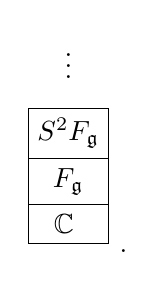
\begin{tikzpicture}[auto,baseline=(current  bounding  box.center)]
\path (0,0) node[name=1, minimum width=1cm, rectangle split, rectangle split parts=3, draw, rectangle split draw splits=true, align=center] 
{ $S^2F_{\fg}$
	\nodepart{two} $F_{\fg}$
	\nodepart{three} $\bC$
} + (0,1.5) node {$\vdots$};
\path (0.7,-0.95) node {$.$};

% \draw (1.text split west) -- (1.text split east);
\end{tikzpicture}  
\end{equation*}
Then the embedding (\ref{eq:skqsubsetsk+1q}) induces embeddings \begin{equation*}
S^kQ_{\fg} \hookrightarrow S^{k+1} Q_{\fg},
\end{equation*} which allow us to define $I_{\fg}$ as the colimit 
\begin{equation*}
I_{\fg}=\varinjlim S^kQ_{\fg}.
\end{equation*} 
Moreover, by the same construction as in Section \ref{subse:intalg}, $I_{\fg}$ is endowed with the structure of a commutative algebra. 

The category $\bT_{\fg}$ is introduced in the same way as in Section \ref{subse:ord-cat}, where now $J_s=W^{\otimes l} \otimes V^{*\otimes m}$ for pairs $s=(l,m)$, $l$, $m\in\bN$, and the object $I$ is replaced by $I_{\fg}$. In the Introduction we denoted this category by $\bT^2_{\fg}$ to emphasize that is generated as a tensor category by two modules $V$ and $V^*$. In the rest of the paper we use the shorter notation $\bT_{\fg}$. We leave it to the reader to check that Proposition \ref{pr.is-ordered} holds also for the category $\bT_{\fg},$  and that $I_{\fg}$ is an injective hull in $\bT_{\fg}$ of the object $\bC$. The respective partial order $(l,m)\preceq (l',m')$ on $\bN\times\bN$ is given by $$l\geq l', \:\:  m\leq m', \:\: l' +m' -l-m = 0 \: (\text{mod 2}). $$ The results of Section \ref{subse:endo} also hold with obvious modification.

The canonical injective resolution (\ref{eq:15}) stays the same with $F$ replaced by $F_{\fg}$, however now the socle of the object $\left(I_{\fg}\right)_j=I_{\fg}\otimes \Lambda^j F_{\fg} $ decomposes as $\bigoplus  \bS_{\lambda} V$ for $\fg=\fs\fp(V)$ and $\bigoplus  \bS_{\lambda^{\perp}} V$ for $\fg=\fo(V)$ where $\lambda$ runs over all special partitions of degree $2j$.

\begin{corollary}
	For any simple object $X$ of $\bT_{\fo(V)}$ we have \begin{equation*}
	\operatorname{Ext}_{\bT_{\fo(V)}}^j (X,\bC)=\begin{cases}	0 \textup{ if }X\not\cong L_{\lambda,\varnothing} \textup{ for  a special } \lambda\textup{  with } |\lambda|=2j, \\ \bC \textup{ if }X\cong L_{\lambda,\varnothing} \textup{ for  a special } \lambda\textup{  with } |\lambda|=2j,
	\end{cases}
	\end{equation*}
	and for any simple object $X$ of $\bT_{\fs\fp(V)}$ we have \begin{equation*}
	\operatorname{Ext}_{\bT_{\fs\fp(V)}}^j (X,\bC)=\begin{cases}	0 \textup{ if }X\not\cong L_{\lambda^{\perp},\varnothing} \textup{ for  a special } \lambda\textup{  with } |\lambda|=2j, \\ \bC \textup{ if }X\cong L_{\lambda^{\perp},\varnothing} \textup{ for  a special } \lambda\textup{  with } |\lambda|=2j.
	\end{cases}
	\end{equation*}
\end{corollary}

Next, Theorem \ref{thm:right-def} and Proposition \ref{pr.thk} stay valid with $\bT$ replaced by $\bT_{\fg}$. We leave it to the reader to modify Lemma \ref{le.exact} accordingly. Furthermore, Proposition \ref{pr:ss}, and Theorem \ref{th:itsimp} also hold for $I_{\fg}$ and $Q_{\fg}$ (instead of $I$ and $Q$, respectively). The same applies to Proposition \ref{pr.itis-ordered}, Theorem \ref{thm:ihulls} (with $L_{\lambda,\mu}$ instead of $L_{\lambda,\mu,\nu,\pi}$), Theorem \ref{th:ikoszcoalg}, Theorem \ref{th:ikosz}, and Corollary \ref{cor.dgradedkoszul}.

The universality results from Section \ref{subse:univ} also carry over to the cases $\fg=\fo(V)$, $\fs\fp(V)$. In particular, the category ${}_{I_{\fg}}\bT$ is defined in the same way as the category ${}_{I}\bT$: it is the category of internal $I_{\fg}$-modules in $\bT_{\fg}$. 

Note also that the analogue \begin{equation*}
V^*\otimes V^* \rightarrow Q_{\fg}\subset I_{\fg}
\end{equation*}
of the map (\ref{eq:partpair}) is well defined and factors through maps \begin{equation*}
S^2V^*\rightarrow Q_{\fg}\text{ and } \Lambda^2V^*\rightarrow Q_{\fg}
\end{equation*}
in the respective cases $\fg=\fo(V)$ and $\fg=\fs\fp(V)$. This defines pairings \begin{equation}\label{eq:igsv}
I_{\fg}\otimes V^* \otimes_{I_{\fg}} \otimes I_{\fg} \otimes V^* \rightarrow I_{\fg} \otimes S^2V^* \rightarrow I_{\fg} 
\end{equation}
and
\begin{equation}\label{eq:iglambdav}
I_{\fg}\otimes V^* \otimes_{I_{\fg}} \otimes I_{\fg} \otimes V^* \rightarrow I_{\fg} \otimes \Lambda^2V^* \rightarrow I_{\fg},
\end{equation}
respectively. 

Now we have 

\begin{theorem}\label{th:osp-univ}
	Let $(\cD,\ \otimes,\ {\bf 1})$ be a tensor category, and $x\hookrightarrow x^*$ be a monomorphism in $\cD$. Assume that a morphism in $\cD$ 
	\begin{equation*}
	p: x^* \otimes x^*\to {\bf 1}
	\end{equation*}
 is given, satisfying $p\circ\sigma=p$ for $\fg=\fo(V)$ and $p\circ\sigma=-p$ for $\fg=\fs\fp(V)$, where $\sigma$ is the flip automorphism of $x^*\otimes x^*$ as an object of the tensor category $\cD$ coming from the assumption that $\cD$ is a symmetric monoidal category.
	\begin{enumerate}[(a)]
		\item There is a unique (up to monoidal natural isomorphism) left exact symmetric monoidal functor $F:{}_{I_{\fg}}\bT_{fin}\to \cD$, where $\fg=\fo(V)$ if $p\circ\sigma=p$ and $\fg=\fs\fp(V)$ if $p\circ\sigma=-p$, sending
		\begin{itemize}
			\item[$-$] the respective pairing (\ref{eq:igsv}) or (\ref{eq:iglambdav}) to $p$;
			\item[$-$] the surjection ${}_{I_{\fg}}V^*\to {}_{I_{\fg}}W$ to $x^*\to x^*/x$.
		\end{itemize}
		\item if $\cD$ is additionally a Grothendieck category then $F$ extends uniquely to a coproduct-preserving functor ${}_{I_{\fg}}\bT\to \cD$.
	\end{enumerate}
\end{theorem}

The universality of the tensor categories ${}_{I_{\fo(V)}}\bT$ and ${}_{I_{\fs\fp(V)}}\bT$ leads to the fact that they are equivalent as monoidal categories. More precisely, consider the (symmetric) tensor category $\bT^-_{\fs\fp(V)}$ defined in the same way as $\bT_{\fs\fp(V)}$ but with the flip isomorphism \begin{equation*}
\sigma: V^*\otimes V^* \rightarrow V^*\otimes V^*,~\sigma(v\otimes w)=w\otimes v
\end{equation*} 
replaced by $-\sigma$. One checks that $\bT^-_{\fs\fp(V)}$ is well-defined, i.e. that the new flip isomorphism on $V^*\otimes V^*$ induces a well-defined structure of tensor category preserving the monoidal structure on $\bT_{\fs\fp(V)}$.

In addition, one checks that there is a well-defined tensor category  ${}_{I_{\fs\fp(V)}}\bT^-$ of internal $I$-modules in $\bT^-_{\fs\fp(V)}$ which coincides with ${}_{I_{\fs\fp(V)}}\bT$ as a monoidal category.

\begin{corollary}
	The tensor categories ${}_{I_{\fo(V)}}\bT$ and ${}_{I_{\fs\fp(V)}}\bT^-$ are canonically equivalent.
\end{corollary}

\begin{proof}
	By Theorem \ref{th:osp-univ}, there are distinguished functors \begin{equation*}
	F:{}_{I_{\fo(V)}}\bT\rightarrow {}_{I_{\fs\fp(V)}}\bT^-
	\end{equation*}
	\begin{equation*}
	F^-:{}_{I_{\fs\fp(V)}}\bT^-\rightarrow {}_{I_{\fo(V)}}\bT
	\end{equation*}
	sending $V^* \otimes I_{\fo(V)}$ to $V^*\otimes I_{\fs\fp(V)}$, $V_* \otimes I_{\fo(V)}$ to $V_* \otimes I_{\fs\fp(V)}$ and $W \otimes I_{\fo(V)}$ to $W \otimes I_{\fs\fp(V)}$, and vice versa. Again, by Theorem \ref{th:osp-univ} the functors $F$ and $F^-$ must be mutually inverse.
	
\end{proof}

%%%%%%%%%%%%%%%%%%%%%%%%%%%%%%%%%%%%%%%%%%%%%%%%%%%%%%%%%%%%%%%%%%%%%%%%%%%%%%%%%%%%%%%%%%%%%%%%%%%%%%%%%%%%%%%%%%
%%%%%%%%%%%%%%%%%%%%%%%%%%%%%%%%%%%%%%%%%%%%%%%%%%%%%%%%%%%%%%%%%%%%%%%%%%%%%%%%%%%%%%%%%%%%%%%%%%%%%%%%%%%%%%%%%%




\bibliography{bib}{}
\bibliographystyle{plain}
\addcontentsline{toc}{section}{References}





\Addresses

\end{document}


